\documentclass[11pt,a4paper]{article}
\usepackage[margin=24mm]{geometry}
\usepackage[T1]{fontenc}
\usepackage{lmodern,microtype,booktabs,longtable,graphicx,xcolor,hyperref}
\definecolor{teal}{HTML}{087E8B}
\hypersetup{colorlinks=true,linkcolor=teal,urlcolor=teal}
\setlength{\emergencystretch}{4em}
\title{IDM-Viz: Consolidated Research Evaluation}
\author{Ahmed Bilal (23I-2581) \and Umar Behram (23I-2604)}
\date{Supplementary research edition, 16 November 2026}
\usepackage{xurl,seqsplit}\setlength{\tabcolsep}{2pt}
\begin{document}
\maketitle
\noindent This corrected edition incorporates the completed robustness replication and has been rendered and visually reviewed page by page. The validation record is included with the report assets.\par

\section{Research basis and scope}

The submitted Phase 2 DOCX is the authoritative methodological basis. No instructor feedback was received. The implementation connects input-distribution alarms, descriptive feature/cluster evidence, source-calibrated current-cohort accuracy estimates, delayed-label verification and coordinated visualization. Its concern score is a plug-in proxy for current-cohort harm relative to historical accuracy; horizon h=0. It is not a validated future-loss forecast. The proposed analyst study, causal discovery and neural anchor remain deferred. The frozen PCA anchor is an explicit substitution. No human benefit is established.\par

The new label-audit comparison is outcome-informed. All existing evidence remains unchanged. Audit actions purchase verification; they do not refit classifiers or increase their accuracy. It evaluates usefulness of automated audit allocation, not analyst decision quality.\par

\section{Equal-budget audit protocol}

Five policies are compared: fixed uniform, input evidence, calibrated concern, conjunction of development-percentile input/concern, and prior released-label evidence. Thresholds use only development seeds 90001-90005. Final seeds 100-129 were already studied, so this is an exploratory extension rather than an untouched confirmatory test. Budget is exactly two or four 500-label cohorts per 24-batch stream. Delays are 0, 5 and 20. Selected predictions precede same-clock release, including zero delay. Remaining quota is filled at the tail, explicitly logged. The released-label comparator makes an initial scheduled probe and may use only selected labels released strictly before the current clock.\par

Equal budget does not imply equal scheduling. Tail filling can favor persistent late drift and hurt recurrence; it is part of the policy, not evidence that an input detector detected a conditional change. The comparison is batch-audit allocation, not episode-level deployment utility. Costs are label counts, not monetary or human costs. Harm targets are model-specific realised accuracy drops greater than 0.05 against the frozen historical reference. Reference uncertainty is omitted.\par

\begin{figure}[htbp]\centering
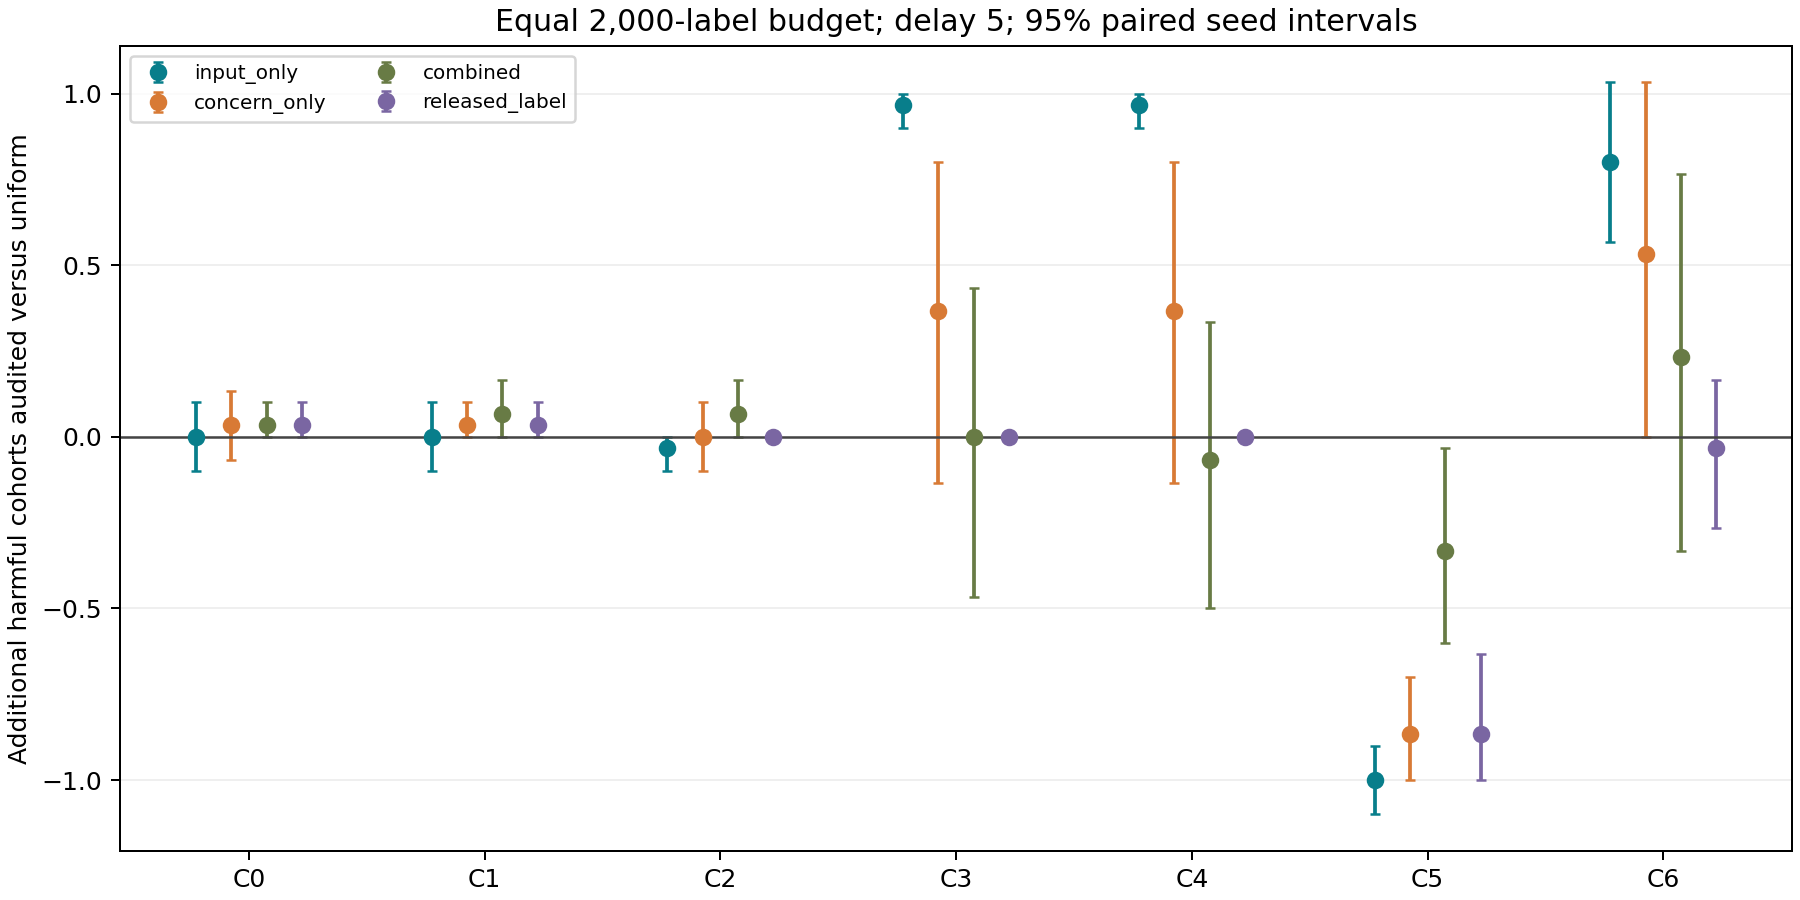
\includegraphics[width=.97\linewidth]{audit_comparison.png}
\caption{Equal-budget comparison}
\end{figure}

\begin{figure}[htbp]\centering
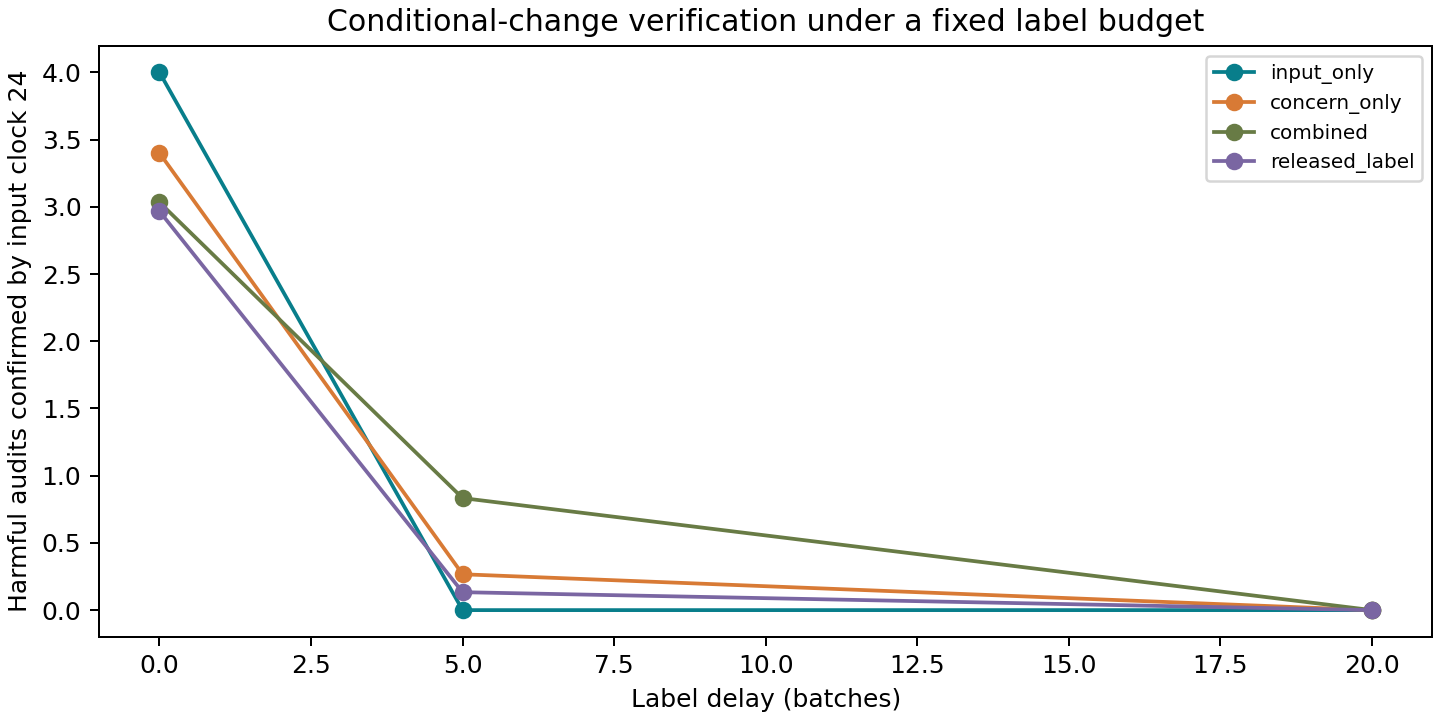
\includegraphics[width=.97\linewidth]{delay_verification.png}
\caption{Delayed verification}
\end{figure}

\section{Paired audit results}

The table includes every condition at the predeclared example delay 5/budget 4. Intervals use 2,000 paired seed bootstrap replicates. These many exploratory comparisons have no familywise significance guarantee; effect sizes are the principal evidence. All delays and budgets are included in the machine-readable results.\par

\begingroup\scriptsize
\begin{longtable}{p{0.182\linewidth}p{0.182\linewidth}p{0.182\linewidth}p{0.182\linewidth}p{0.182\linewidth}}
\toprule
condition & policy & mean & lower & upper \\
\midrule
\endfirsthead
\toprule
condition & policy & mean & lower & upper \\
\midrule
\endhead
C0 & input\_\allowbreak{}only & 0.000 & -0.100 & 0.100 \\
C0 & concern\_\allowbreak{}only & 0.033 & -0.067 & 0.133 \\
C0 & combined & 0.033 & 0.000 & 0.100 \\
C0 & released\_\allowbreak{}label & 0.033 & 0.000 & 0.100 \\
C1 & input\_\allowbreak{}only & 0.000 & -0.100 & 0.100 \\
C1 & concern\_\allowbreak{}only & 0.033 & 0.000 & 0.100 \\
C1 & combined & 0.067 & 0.000 & 0.167 \\
C1 & released\_\allowbreak{}label & 0.033 & 0.000 & 0.100 \\
C2 & input\_\allowbreak{}only & -0.033 & -0.100 & 0.000 \\
C2 & concern\_\allowbreak{}only & 0.000 & -0.100 & 0.100 \\
C2 & combined & 0.067 & 0.000 & 0.167 \\
C2 & released\_\allowbreak{}label & 0.000 & 0.000 & 0.000 \\
C3 & input\_\allowbreak{}only & 0.967 & 0.900 & 1.000 \\
C3 & concern\_\allowbreak{}only & 0.367 & -0.133 & 0.800 \\
C3 & combined & 0.000 & -0.467 & 0.433 \\
C3 & released\_\allowbreak{}label & 0.000 & 0.000 & 0.000 \\
C4 & input\_\allowbreak{}only & 0.967 & 0.900 & 1.000 \\
C4 & concern\_\allowbreak{}only & 0.367 & -0.134 & 0.800 \\
C4 & combined & -0.067 & -0.500 & 0.333 \\
C4 & released\_\allowbreak{}label & 0.000 & 0.000 & 0.000 \\
C5 & input\_\allowbreak{}only & -1.000 & -1.100 & -0.900 \\
C5 & concern\_\allowbreak{}only & -0.867 & -1.000 & -0.700 \\
C5 & combined & -0.333 & -0.600 & -0.033 \\
C5 & released\_\allowbreak{}label & -0.867 & -1.000 & -0.633 \\
C6 & input\_\allowbreak{}only & 0.800 & 0.567 & 1.033 \\
C6 & concern\_\allowbreak{}only & 0.533 & 0.000 & 1.033 \\
C6 & combined & 0.233 & -0.333 & 0.767 \\
C6 & released\_\allowbreak{}label & -0.033 & -0.267 & 0.167 \\
\bottomrule
\end{longtable}
\endgroup

\section{Feature-localization evidence}

\begingroup\scriptsize
\begin{longtable}{p{0.2275\linewidth}p{0.2275\linewidth}p{0.2275\linewidth}p{0.2275\linewidth}}
\toprule
condition & precision\_\allowbreak{}at\_\allowbreak{}1 & recall\_\allowbreak{}at\_\allowbreak{}3 & feature\_\allowbreak{}flag\_\allowbreak{}recall \\
\midrule
\endfirsthead
\toprule
condition & precision\_\allowbreak{}at\_\allowbreak{}1 & recall\_\allowbreak{}at\_\allowbreak{}3 & feature\_\allowbreak{}flag\_\allowbreak{}recall \\
\midrule
\endhead
C1 & 1.000 & 1.000 & 1.000 \\
C2 & 0.988 & 0.994 & 0.973 \\
\bottomrule
\end{longtable}
\endgroup

These values are aggregated over batches with known changed marginals in C1/C2. They are not causal attribution. C6 changes dependence with unchanged marginals; C3-C5 alter labels without a known changed input marginal. Their feature-localization metric is undefined, not zero or successful. Frozen clusters are descriptive regions, not validated causal explanations.\par

\section{External calibration transfer failure}

The preserved UCI 224 cohort evaluation uses batch 1 split into 267 training, 89 calibration and 89 reference rows; batches 2-10 remain whole monitoring cohorts. Mean cohort accuracy is 0.432, macro-F1 0.290, calibrated estimated accuracy 0.976, MAE 0.545, approximate interval coverage 0/9 and input alarms 9/9. This is one external dataset and not nine independent replications. Class composition and sensor conditions change together. Small source calibration, normal-approximation intervals, a different correctness mapping and absent simulated release timing limit comparability with the synthetic study. Historical batch-1 class-proportion metadata has a denominator defect; monitoring outcomes are unaffected, but that metadata must not be used as a probability distribution. The class-mix sensitivity is descriptive and outcome-informed.\par

\section{Research comparison and interpretation}

Average Thresholded Confidence predicts target accuracy using thresholded model confidence. Garg et al. show that unlabeled accuracy estimation requires assumptions about distribution shift; comparison to their published numeric scores is not fair on our different generators and learners. Our ATC-style baseline is therefore a within-study comparator. Ovadia et al. benchmark uncertainty under dataset shift, supporting evaluation of calibration transfer rather than an assumption that source calibration persists. Neither paper establishes IDM-Viz's superiority or analyst usefulness. Sources: \url{https://arxiv.org/abs/2201.04234} and \url{https://proceedings.neurips.cc/paper/2019/hash/8558cb408c1d76621371888657d2eb1d-Abstract.html} .\par

\section{Original and model/task extension evidence}

The following preserved study text supplies the classifier setup, baseline and component-ablation evidence. It predates the audit extension; its scope statements refer to that study version. Timings and historical receipts must not be presented as newly repeated tests.\par



\section{Model/task study}


Ahmed Bilal (23I-2581) and Umar Behram (23I-2604)\par
Department of AI and Data Science, FAST-NUCES Islamabad\par
Data Analysis and Visualization\par

Protocol status: Outcome-informed extension; final evidence generated from the locked extension protocol.\par

\section{Summary}

Version 2 adds a fixed shallow tree comparison on the original controlled task and a new XOR synthetic task. The final run has 360 feature streams and 17,280 model-batch records. It evaluates both learners with their own correctness calibrator, ATC-style threshold and historical reference. The XOR task is synthetic and is not external-domain validation.\par

On stationary XOR, tree minus logistic accuracy was 0.2168 (seed-bootstrap 95\% interval 0.1567 to 0.2751). On v1 stationary data the paired accuracy difference was -0.0323 (-0.0343 to -0.0301).\par

Exact extension check passed for 210 v1-task streams, 1680 cached arrays and 25,210,080 array values. V1 logistic predictions, confidence arrays and original condition records are preserved as the matched comparison; no v1 seed or outcome is replaced.\par

\section{What the extension tests}

The shallow tree is fixed at Gini criterion, depth 6 and minimum leaf size 25. Logistic regression retains \texttt{\seqsplit{C=1}}, \texttt{\seqsplit{max\_\allowbreak{}iter=500}} and a 0.5 class cutoff. Both models use training-only scaling and independent isotonic calibrators fitted on the same correctness-calibration rows. No hyperparameter search is performed.\par

The new XOR task uses eight independent standard-normal features and the noisy concept \texttt{\seqsplit{1\{(X0 > 0) XOR (X1 > 0)\}}} with 10\% baseline label noise. Its locked interventions are stationary, irrelevant mean shift, relevant mean shift, concept complement and increased label noise. The last two preserve inputs and alter only the label law. Synthetic event times are known from construction; no onset labels are fabricated for a natural dataset.\par

The local ELEC2 candidate was rejected: the raw ARFF's \texttt{\seqsplit{date}} is non-monotone, 528 \texttt{\seqsplit{(date, period)}} pairs repeat, and 11 date values have 96 rows instead of 48. The date/period fields therefore do not uniquely reconstruct row chronology. The processed parquet also fails to read. OpenML's local metadata reports its license field as \texttt{\seqsplit{Public}}; this report does not turn that label into a specific permissive license. The source record and original study are listed at the end.\par

\section{Overall results}

\begingroup\scriptsize
\begin{longtable}{p{0.182\linewidth}p{0.182\linewidth}p{0.182\linewidth}p{0.182\linewidth}p{0.182\linewidth}}
\toprule
Task & Model & Calibrated AC MAE, mean [seed-bootstrap 95\% interval] & Coverage & Mean interval width \\
\midrule
\endfirsthead
\toprule
Task & Model & Calibrated AC MAE, mean [seed-bootstrap 95\% interval] & Coverage & Mean interval width \\
\midrule
\endhead
Original synthetic task & Logistic & 0.114189 [0.113086, 0.115365] & 0.695238 [0.675397, 0.712103] & 0.073760 [0.073481, 0.074024] \\
Original synthetic task & Shallow tree & 0.105031 [0.103582, 0.106560] & 0.622817 [0.605754, 0.639484] & 0.077718 [0.077465, 0.077968] \\
XOR synthetic task & Logistic & 0.023147 [0.021421, 0.024964] & 0.876667 [0.852771, 0.900833] & 0.087413 [0.087353, 0.087474] \\
XOR synthetic task & Shallow tree & 0.089146 [0.069485, 0.110378] & 0.750278 [0.705826, 0.798618] & 0.069385 [0.063868, 0.074830] \\
\bottomrule
\end{longtable}
\endgroup

For context, the earlier study reported calibrated AC MAE 0.114189 versus raw AC MAE 0.113387, and calibrated coverage 0.695238. Its retained baseline tables give the corresponding seed rows and denominators. These cohorts are not pooled with the two new synthetic tasks.\par

Per-condition summaries, complete seed rows, paired seed contrasts, pooled harm counts, undefined metrics and bootstrap intervals are provided in the CSV files. The tree's model-specific historical reference changes its realised-harm label; differences in harm counts alone do not rank the models. Matched-cohort accuracy and estimation error are reported separately.\par

\section{Failure analysis}

In v1 C3-C5, the calibrated confidence channel averaged 0.723 while evaluator-only accuracy averaged 0.488; 1,205 batches met the v1 realised-harm rule and the calibrated concern rule flagged 0. This is measured. Those conditions reuse identical input arrays while changing the conditional label law, so the input detector has no distributional input evidence by construction. The model receives familiar inputs and retains its source confidence even when its predictions become wrong. The frozen source calibrator cannot infer a label-law reversal from confidence alone.\par

Version 1 calibrated AC MAE (0.114189) exceeded raw AC MAE (0.113387) by 0.000802; calibrated interval coverage was 0.695. The plausible explanation that an isotonic map learned source reliability but did not transfer to changed regimes is consistent with the conditional-only results, but it is not a unique causal explanation. V2 adds pre/onset/post/recovery reliability summaries and reports calibration error and Brier score by model and regime.\par

For C6, v1 matched the dependence onset in 8/30 seeds with full KS/PCA and 4/30 with original-feature KS. Individual frozen PCA-coordinate adjusted-p detections in the onset window were: PC0 6/30, PC1 1/30, PC2 0/30. PCA therefore supplied some additional task-specific marginal evidence, but did not solve the missed-event problem; the PCA basis is descriptive and fixed from training.\par

Version 2 reports interval width alongside empirical coverage and concern TP/FP/FN/TN counts for each task, model, condition and regime. A no-flag outcome is not a safety verdict. The plug-in Poisson-binomial interval and concern score are not calibrated harm probabilities or arbitrary-shift coverage guarantees.\par

At the end of 24 input batches, delayed verification leaves 0 batches unresolved for delay 0, 5 for delay 5, and 20 for delay 20; after drainage all 24 are verified at ages 0, 5 and 20 batches respectively. Delay changes evidence availability and age, not the frozen estimator's accuracy.\par

\section{Figures}

Paired model sensitivity: estimation error by task, condition and learner.\par

\begin{figure}[htbp]\centering
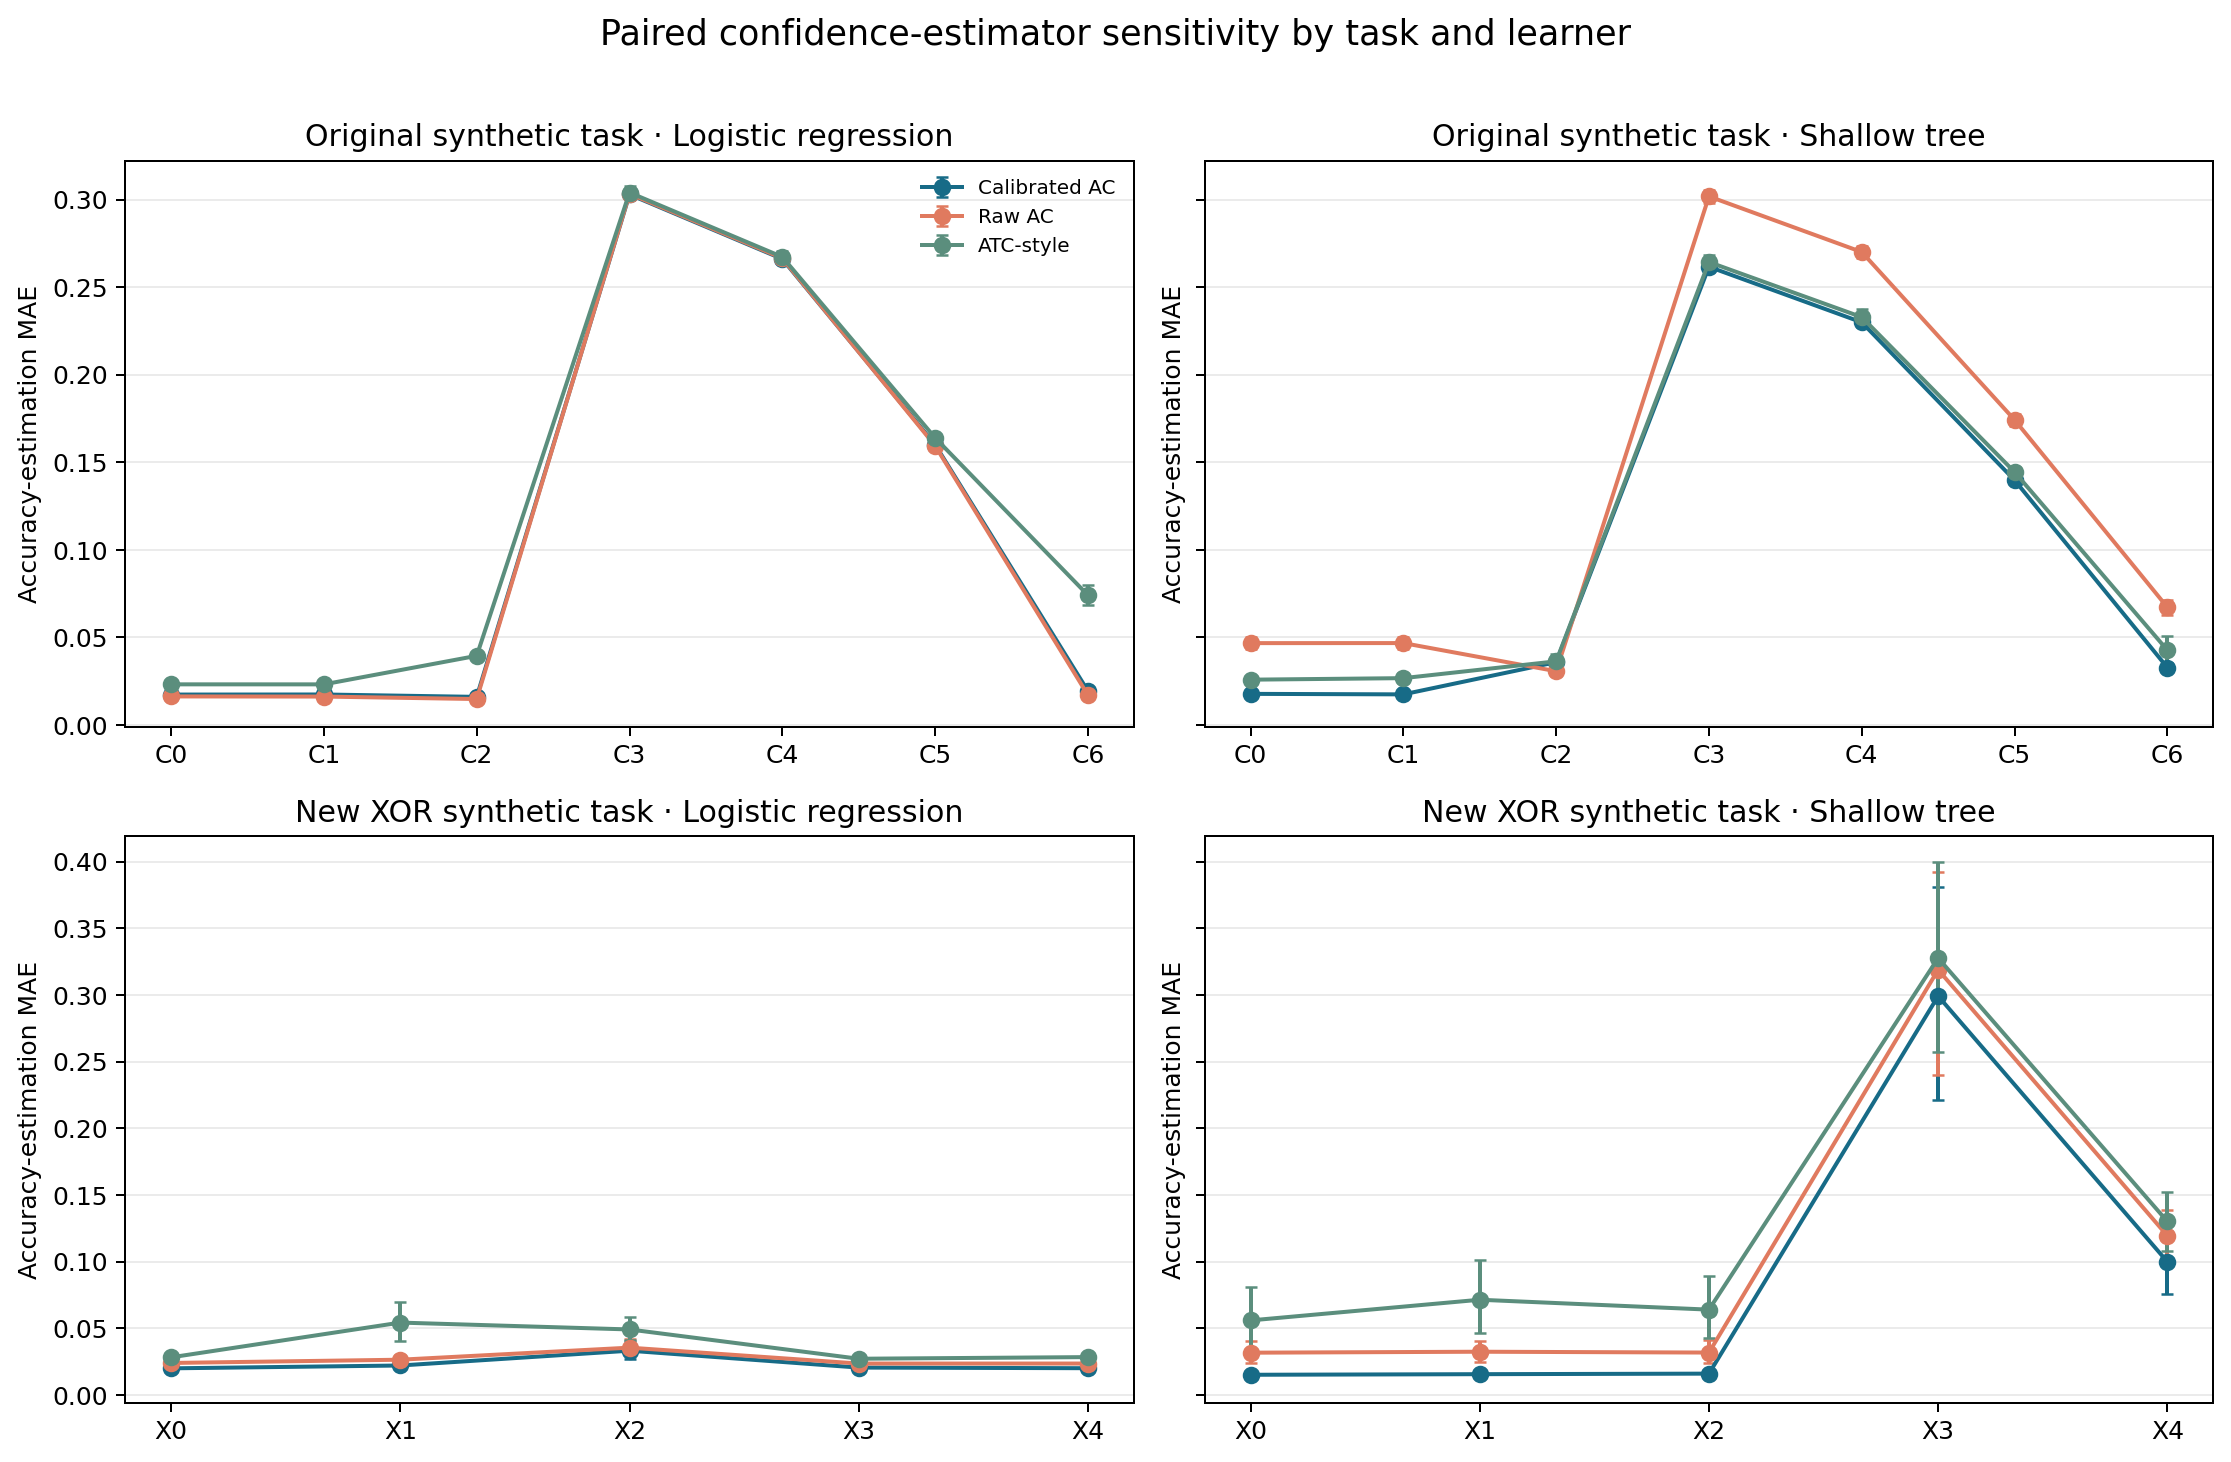
\includegraphics[width=.97\linewidth]{preserved_0_model_sensitivity_mae.png}
\caption{Paired model sensitivity}
\end{figure}

Interval behavior: empirical coverage and width; the nominal line is a target.\par

\begin{figure}[htbp]\centering
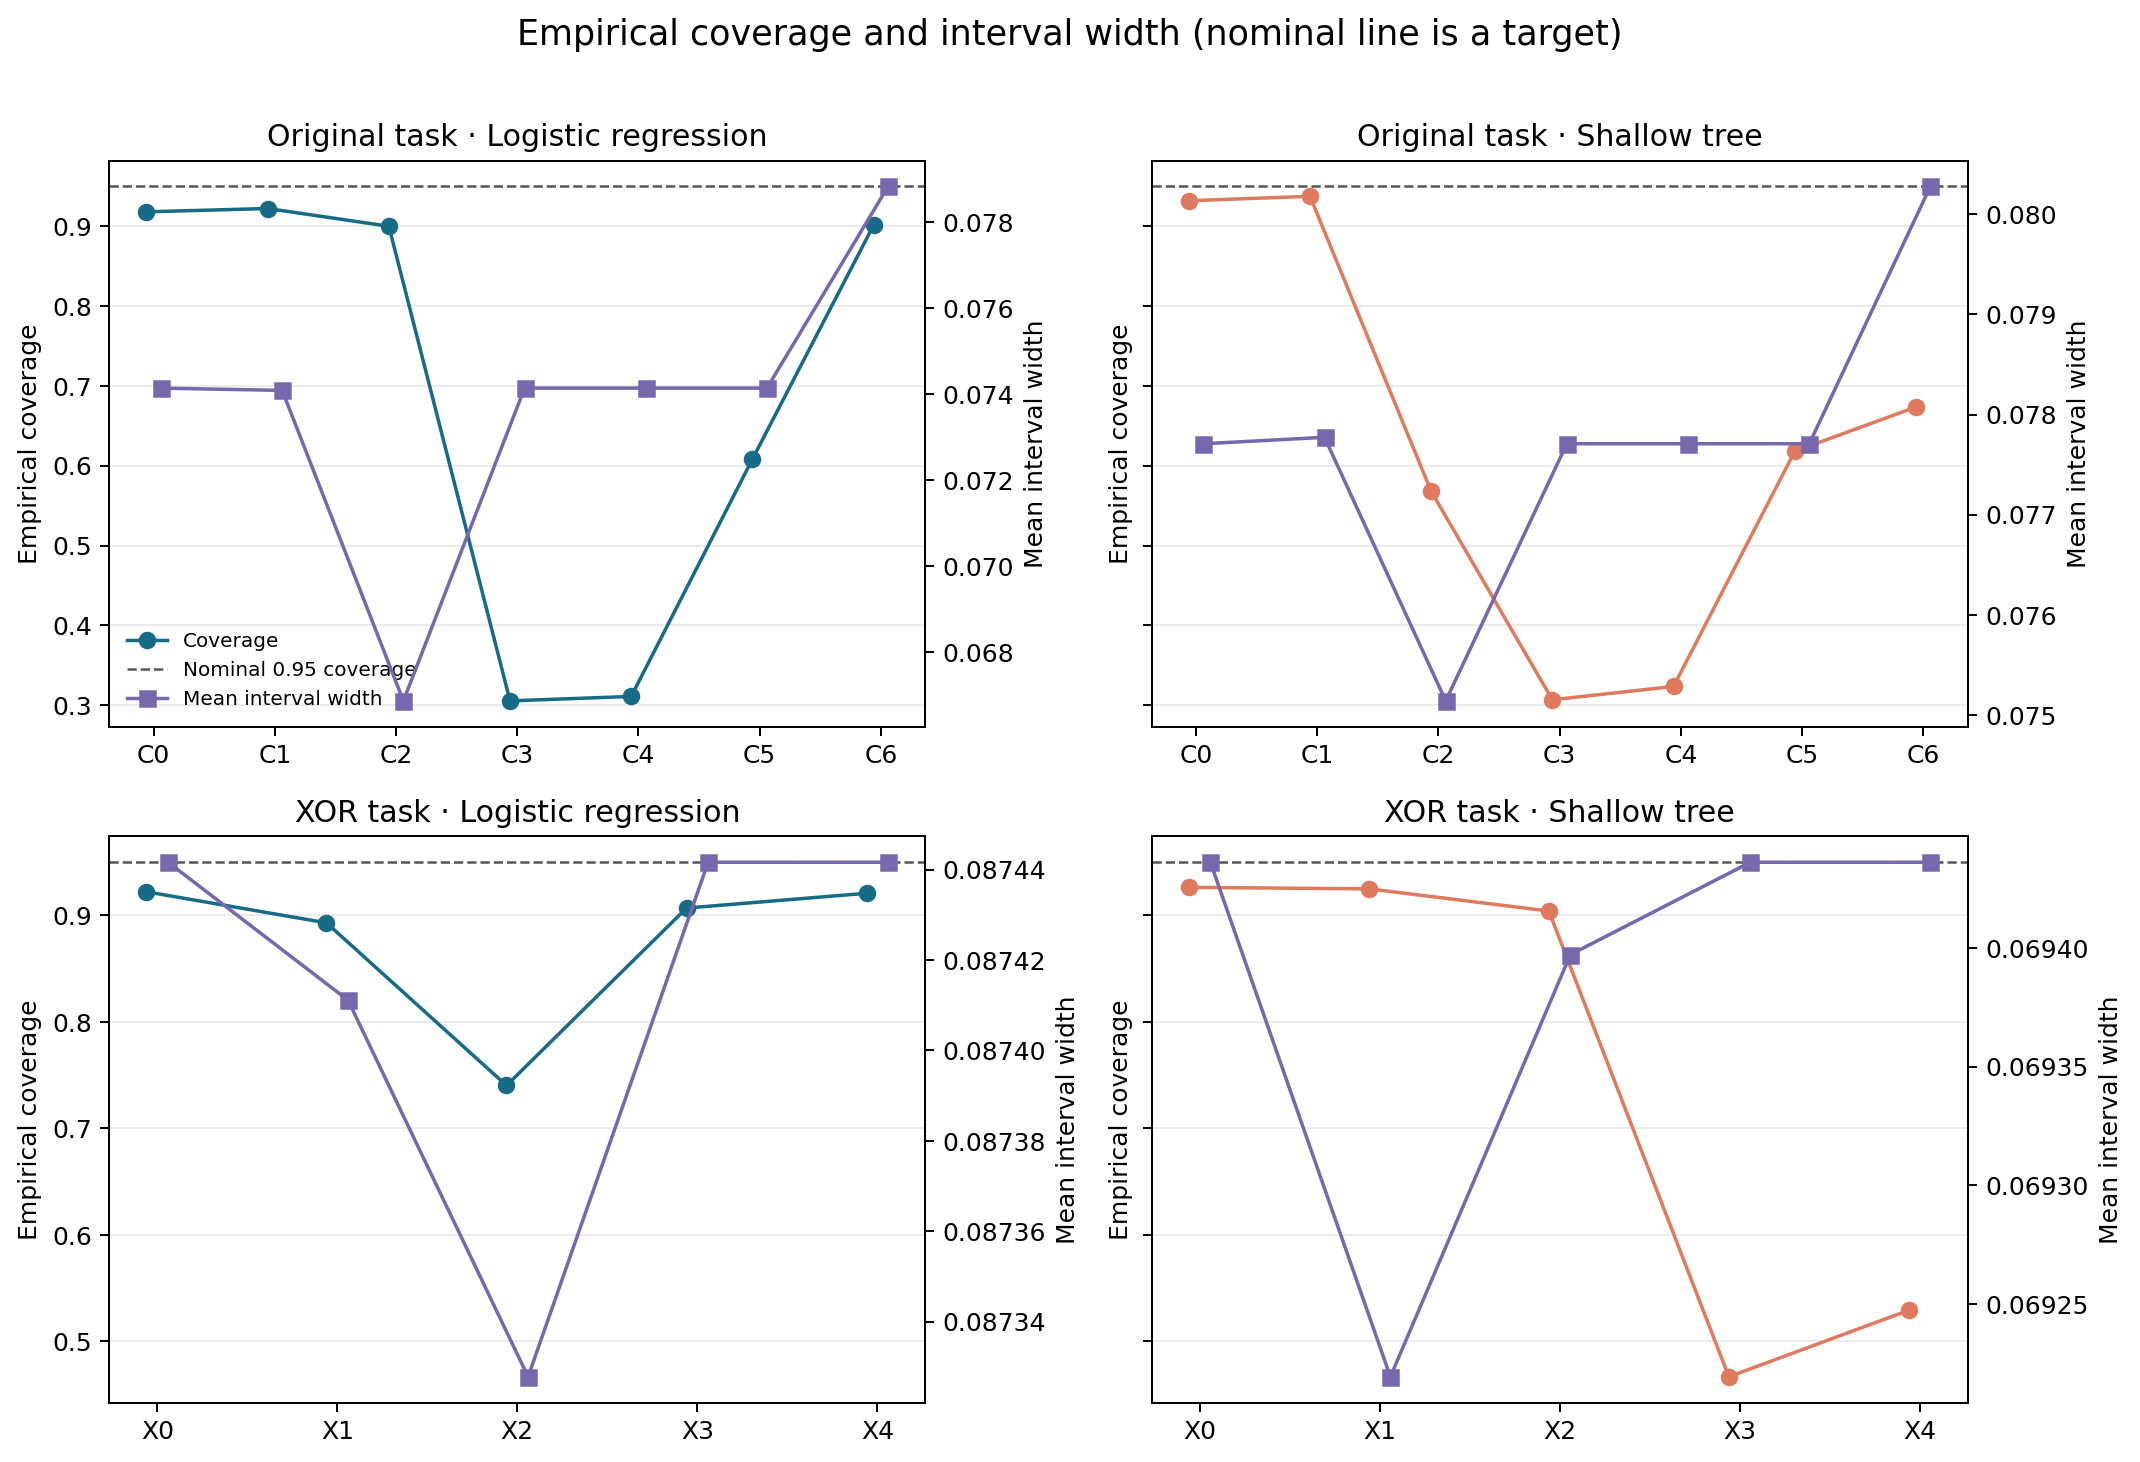
\includegraphics[width=.97\linewidth]{preserved_0_interval_coverage_width.png}
\caption{Coverage and interval width}
\end{figure}

Concern-rule outcomes: harmful batches left unflagged are shown directly.\par

\begin{figure}[htbp]\centering
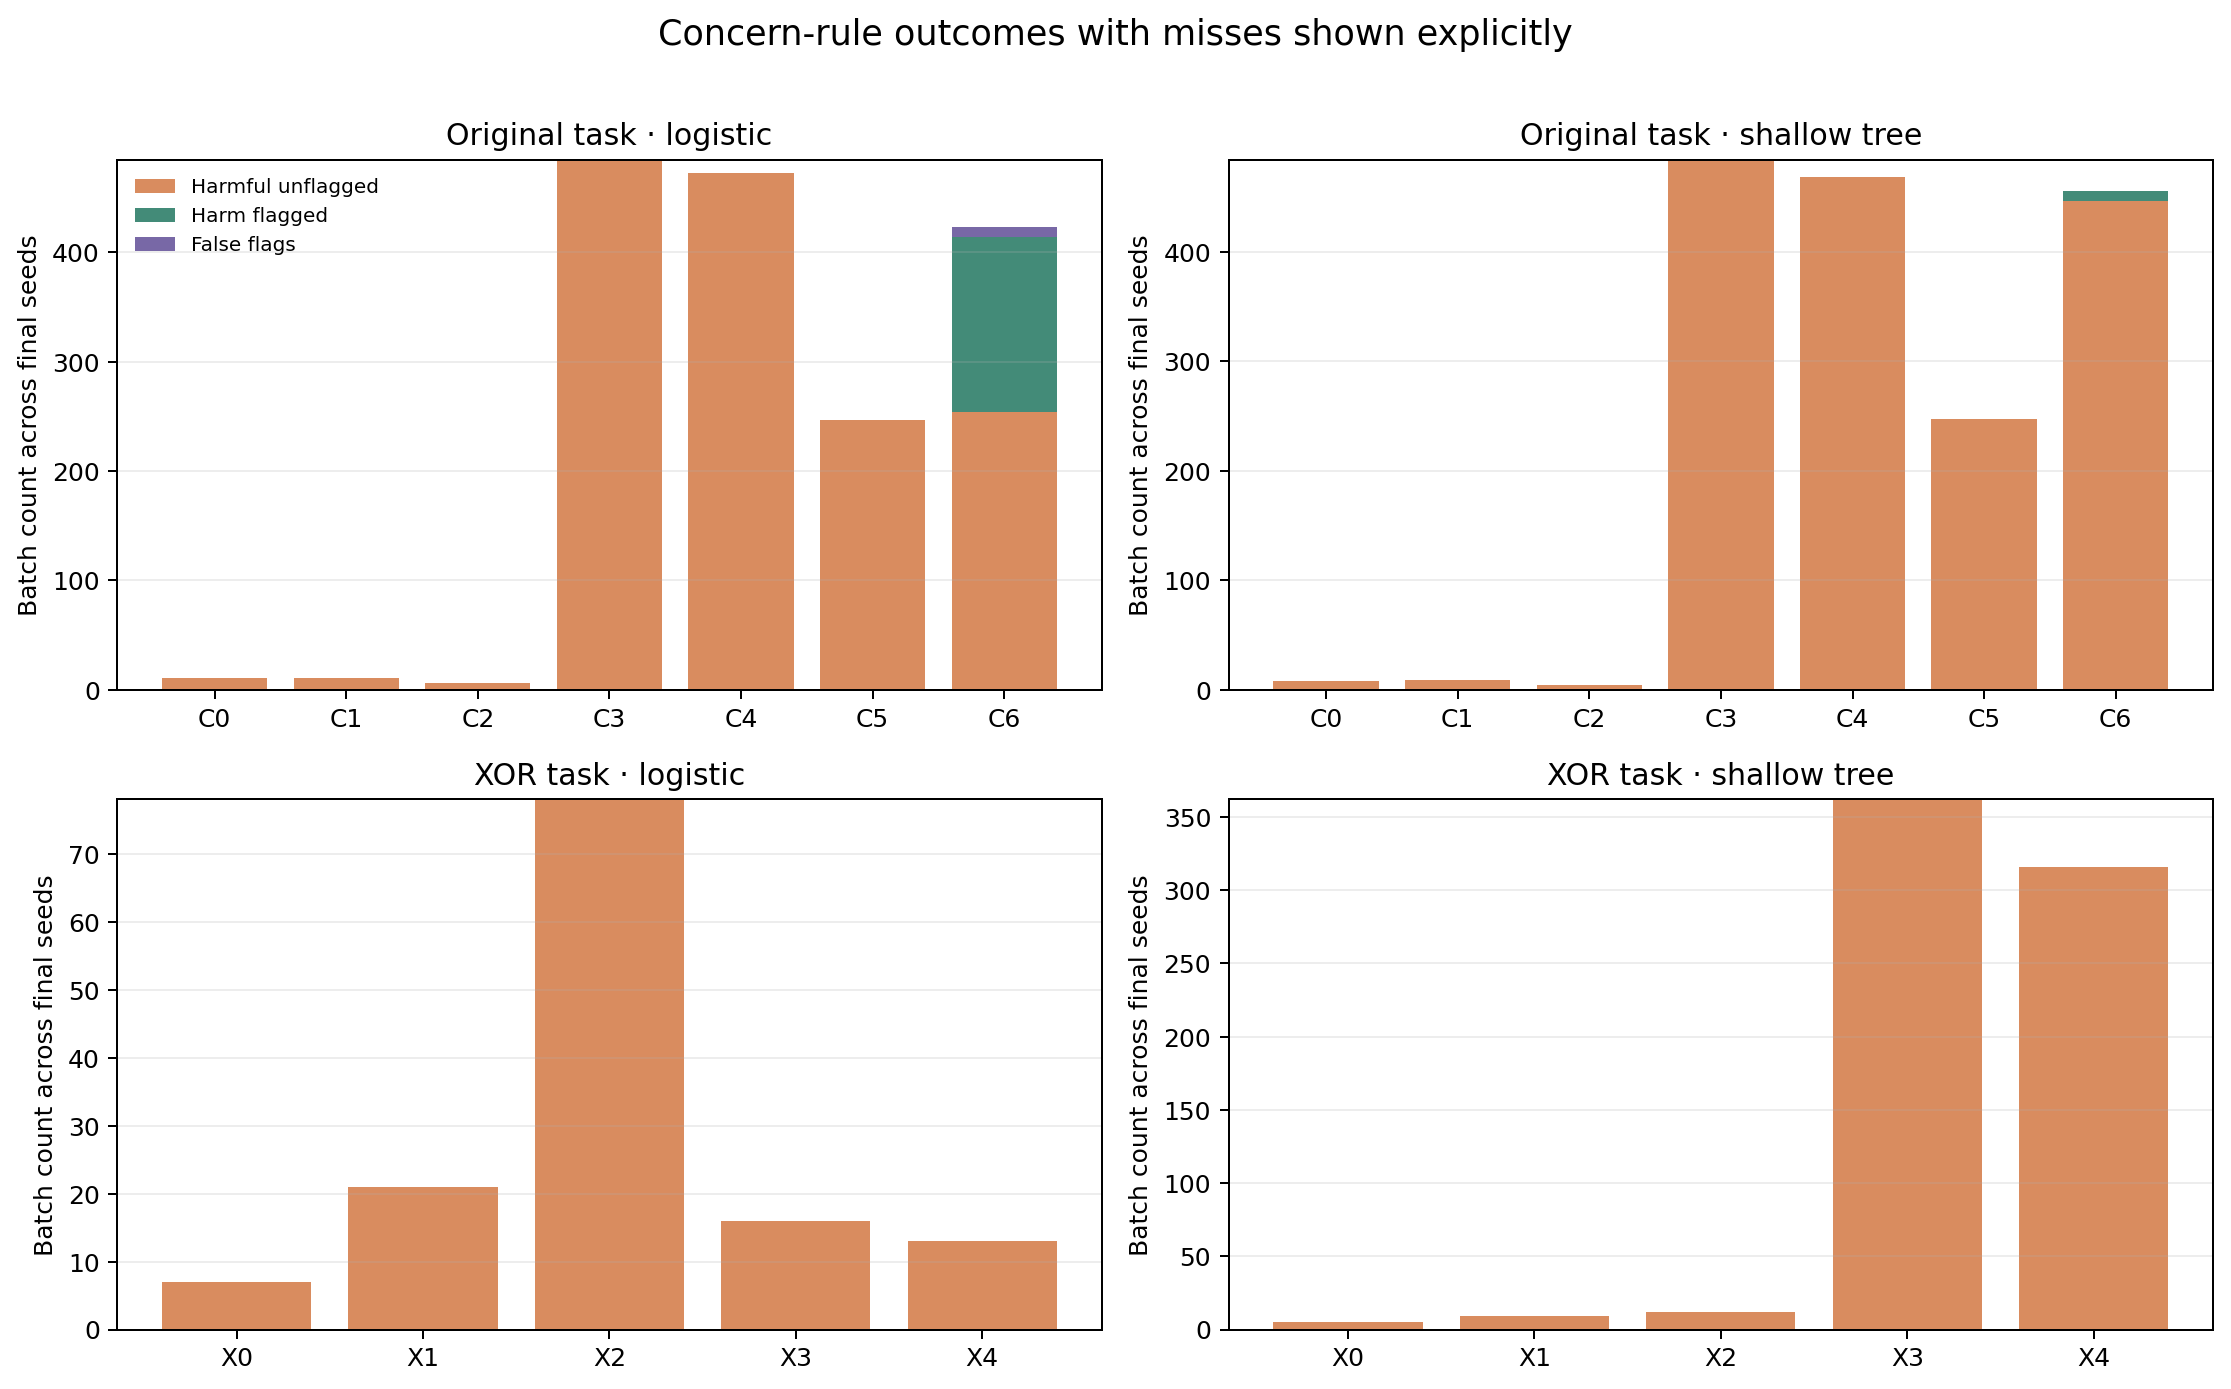
\includegraphics[width=.97\linewidth]{preserved_0_harm_concern_outcomes.png}
\caption{Harm flags and misses}
\end{figure}

Reliability: calibrated and raw scores across stream regimes.\par

\begin{figure}[htbp]\centering
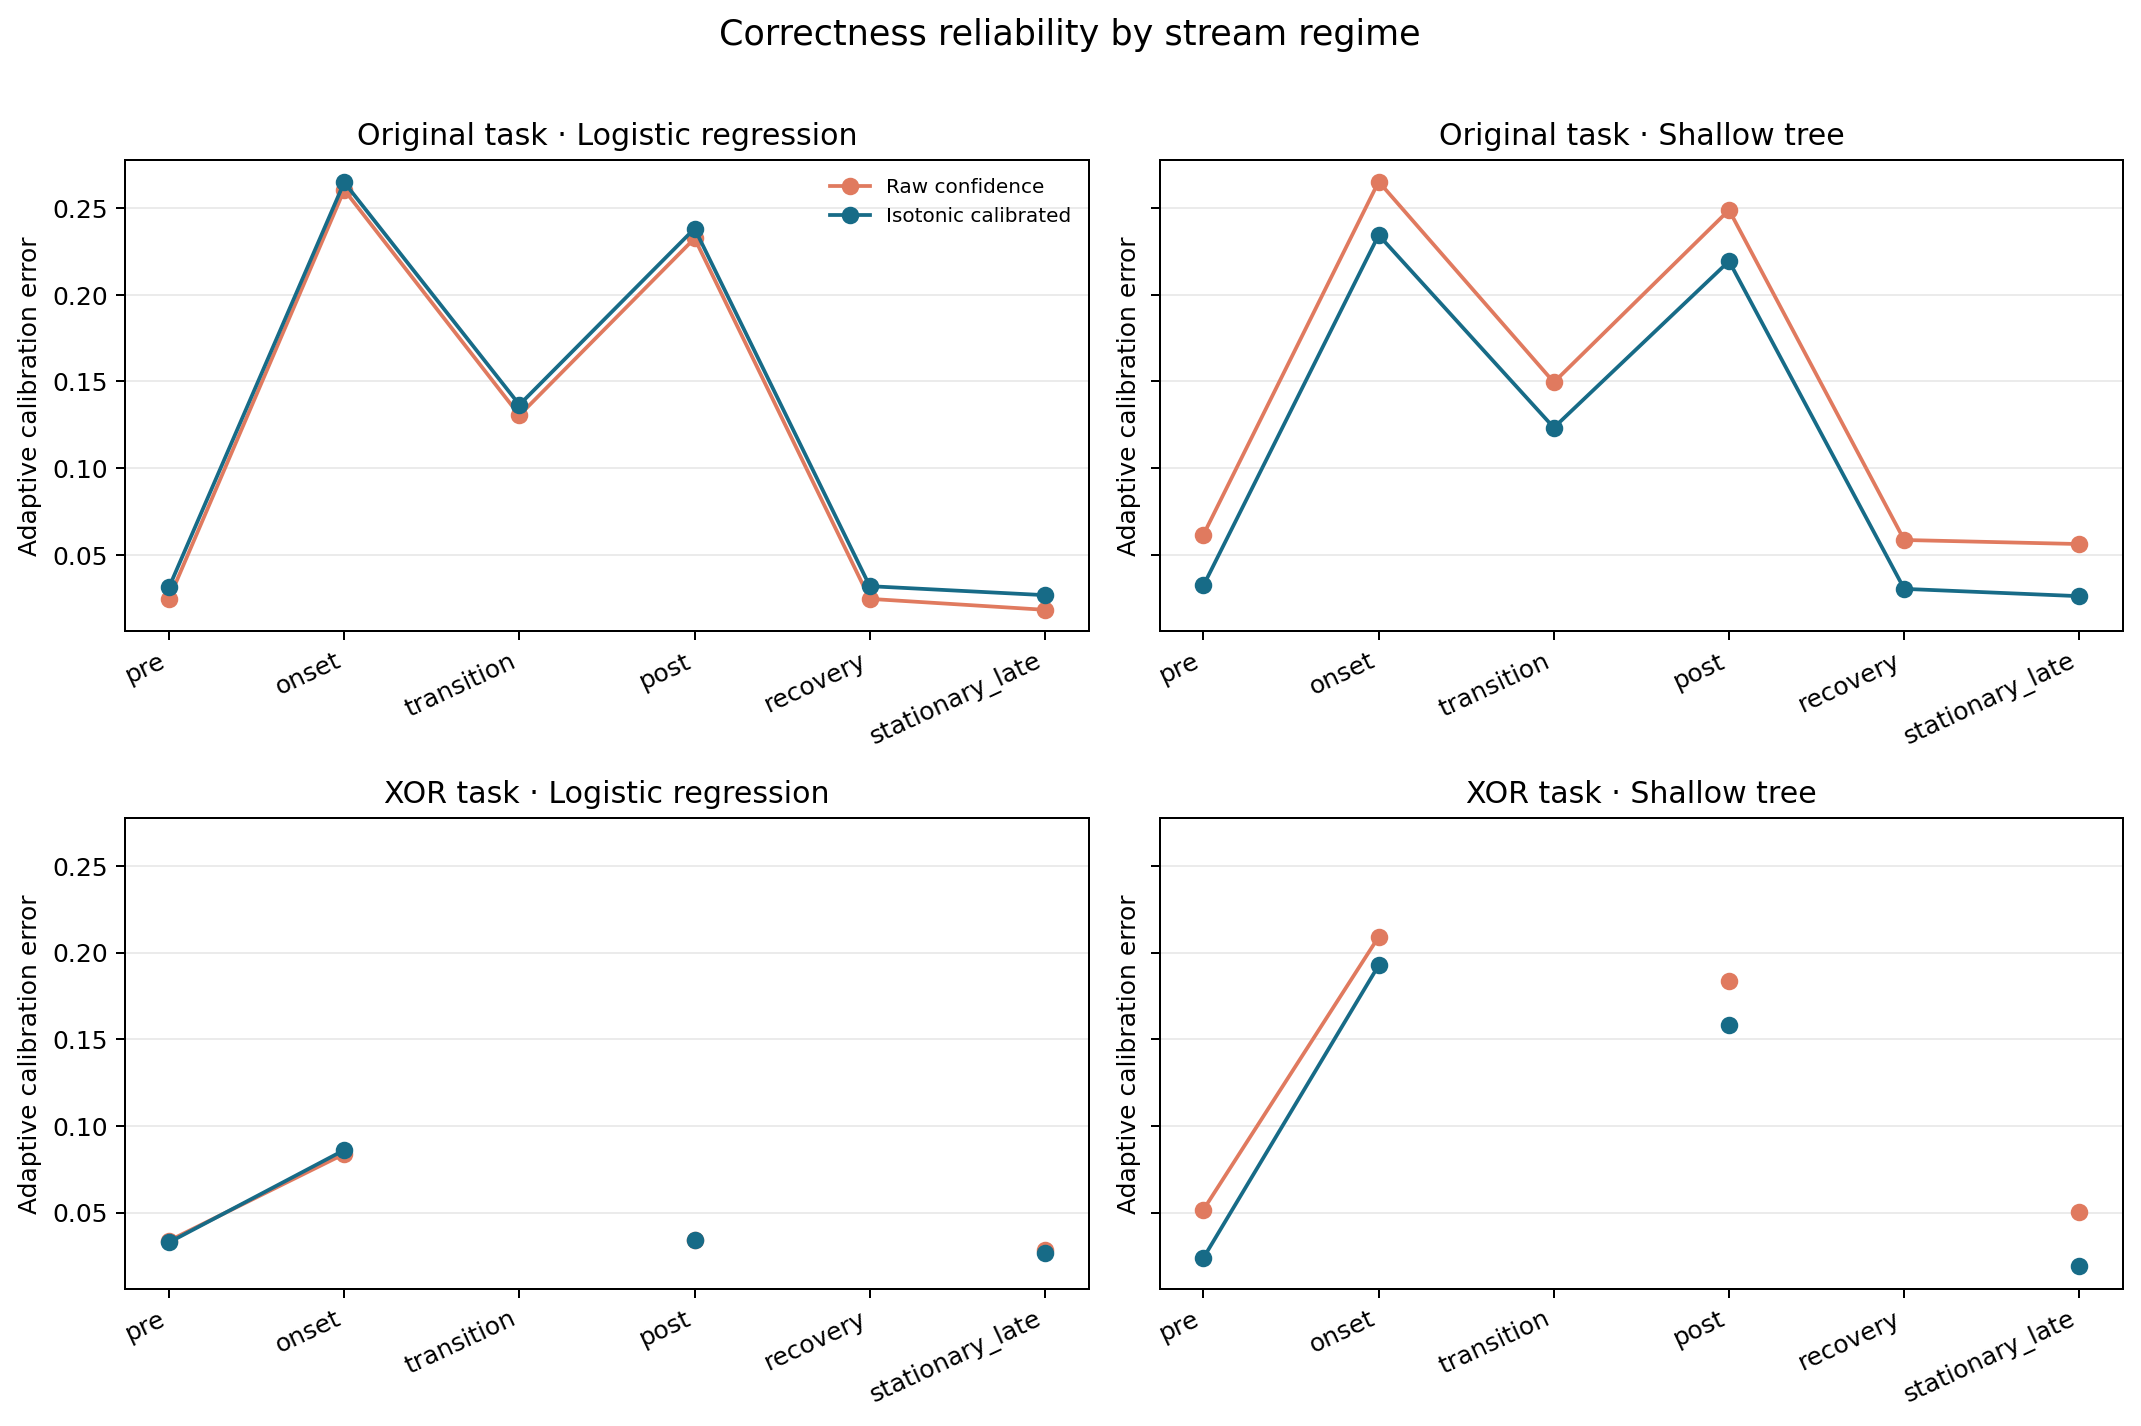
\includegraphics[width=.97\linewidth]{preserved_0_calibration_by_regime.png}
\caption{Calibration by regime}
\end{figure}

V1 failure analysis: conditional-only shift with evaluator-only truth.\par

\begin{figure}[htbp]\centering
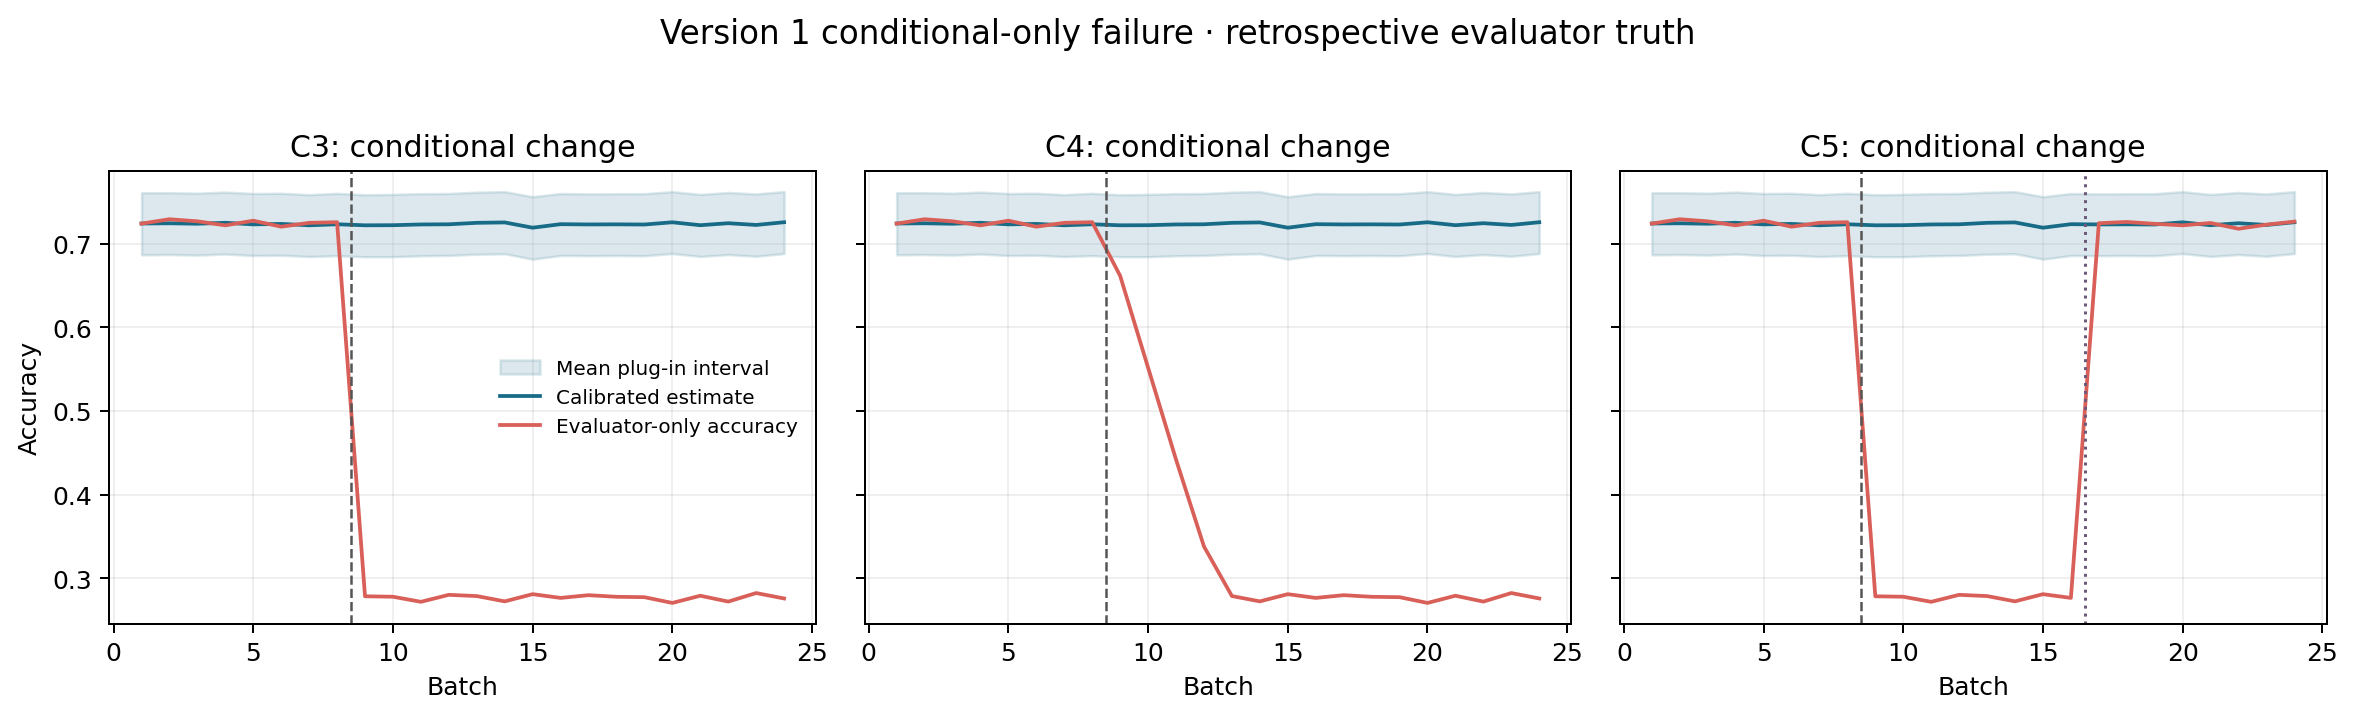
\includegraphics[width=.97\linewidth]{preserved_0_v1_conditional_failure.png}
\caption{Conditional-only failure}
\end{figure}

V1 dependence analysis: adjusted-p detections by frozen PCA coordinate.\par

\begin{figure}[htbp]\centering
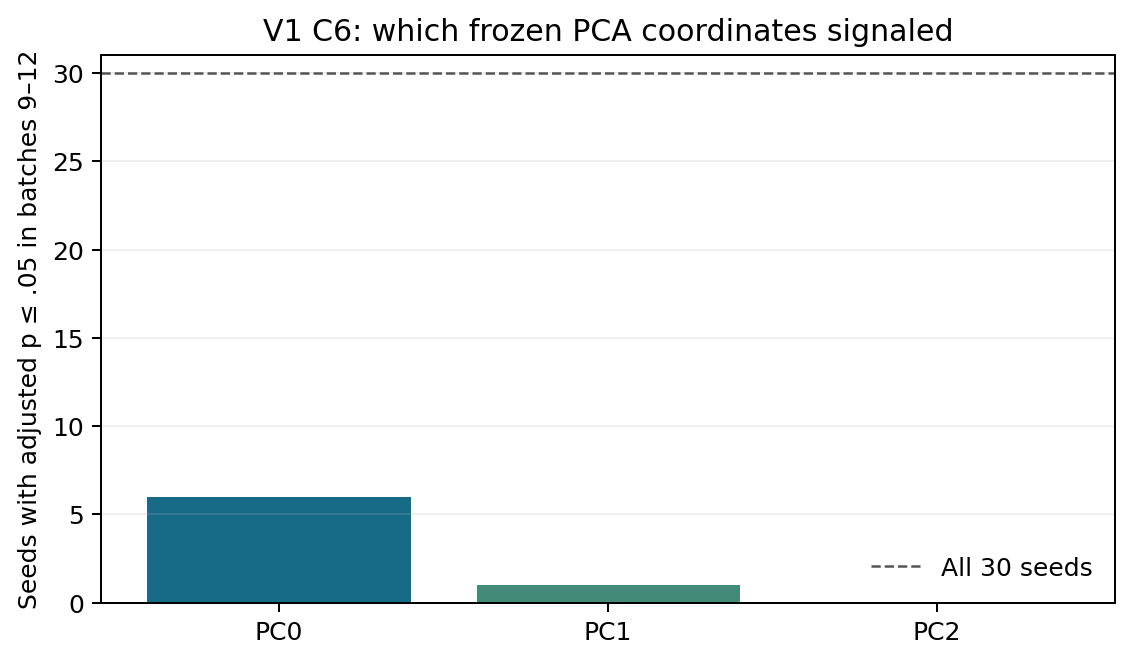
\includegraphics[width=.97\linewidth]{preserved_0_v1_c6_pca_components.png}
\caption{Dependence coordinate detection}
\end{figure}


\section{Version comparison and research questions}

- Established beyond v1: model sensitivity on matched original-task observations; an independently seeded synthetic task with an axis-aligned nonlinear boundary; model-specific calibration, harm targets, intervals and paired uncertainty; failure reliability split by task, model and regime.\par
- Contradicts a universal model claim: neither learner dominates every task/regime on accuracy, estimation error, coverage and harm flags. Interpret comparisons only within matched cohorts and state the model-specific reference target.\par
- Unchanged: v1's logistic method, original condition evidence, thresholds, delays and negative findings remain intact. V2 does not retrofit v1 outcomes or claim a natural-domain replication.\par
- RQ1: current-batch realised deterioration is evaluated in controlled synthetic streams; future forecasting and certified population harm remain untested.\par
- RQ2: feature evidence remains descriptive marginal ranking; causal attribution and cluster localization accuracy remain unanswered.\par
- RQ3: analyst benefit remains unanswered; there is no human-subject evaluation.\par
- RQ4: robustness evidence now spans two synthetic task families, not external or natural-domain validation.\par

\section{Limitations and provenance}

The evidence uses one linear probabilistic learner and one fixed shallow tree on two synthetic families. It does not include external-domain validation, neural autoencoders, causal discovery, online adaptation, selective-label analysis or a human study. Calibration is frozen, confidence-based, and dependent on the source law. Interval width and empirical coverage are descriptive. Bootstrap intervals resample complete seed vectors; batches, delay copies, models and ablations are not treated as independent datasets. Version 2 hypotheses were informed by observed v1 outcomes, so the extension is not described as an untouched preregistration.\par

The submitted Phase 2 DOCX remains the methodological basis; the older TeX is only supporting material, and no instructor feedback was received. The original two-page implementation brief was consulted and preserved. The existing offline replay is a prototype, contains retrospective release information and is not a security boundary or human-evaluation result.\par

Sources consulted for the rejected ELEC2 candidate: [OpenML dataset 151](\url{https://www.openml.org/d/151);} Gama, Medas, Castillo and Rodrigues, *Learning with Drift Detection* (2004), [primary paper](\url{https://sweet.ua.pt/gladys/Papers/GamaMedasCastilloRodriguesSBIA04.pdf)} The published task results are not treated as comparable benchmarks.\par

\section{Reproduction and artifact semantics}

Independent reproduction: a clean run matched 741 CSVs (6,768,744 cells) and 1,140 compressed arrays (6,660 arrays; 95,554,560 values) exactly. Timing columns and protocol metadata were excluded from scientific equality checks.\par
The first comparator attempt differed only in bootstrap summaries of wall-clock \texttt{\seqsplit{input\_\allowbreak{}seconds}}. That engineering timing was removed from uncertainty summaries, and both saved runs were reevaluated; no inputs, seeds, predictions, model settings or scientific thresholds changed.\par

Use \texttt{\seqsplit{Reproduce.md}} for the package contents and run separation; the project workspace guide \texttt{\seqsplit{docs/phase3/23I-2581\_\allowbreak{}23I-2604\_\allowbreak{}Phase3\_\allowbreak{}Reproduction.md}} gives the exact full-rerun commands. The final run has a protocol lock and exact environment versions. \texttt{\seqsplit{predictions/}} contain persisted online scores; \texttt{\seqsplit{released\_\allowbreak{}verification.csv}} contains scheduled label results; \texttt{\seqsplit{evaluator\_\allowbreak{}truth/}} and \texttt{\seqsplit{evaluator\_\allowbreak{}batches.csv}} are retrospective. Historical source documents and run archives are preserved.\par


\section{Selected adaptation study}


Ahmed Bilal (23I-2581) and Umar Behram (23I-2604)\par
Data Analysis and Visualization · Phase 3 supplementary experiment\par

Status: Outcome-informed exploratory add-on, protocol locked before its development and final runs.\par

\section{Question and scope}

This small experiment asks whether cumulative refitting on labels after their scheduled release changes batch accuracy under two selected synthetic conditional changes: C3 (label-probability reversal with unchanged inputs) and X3 (XOR concept complement with unchanged inputs). Selection was informed by the earlier study's conditional-only failures and the extension's XOR task. The experiment is not external validation and is kept separate from the frozen-model results.\par

This final evidence uses 30 seeds per condition, 3 delays, and 24 batches of 500 rows. It created 60 feature streams, 180 delay streams, 8640 online method-batch records, 4,320,000 exact prediction/truth joins and 2,160,000 scheduled label rows.\par

\section{Locked comparison}

Both arms use LogisticRegression(C=1, max\_\allowbreak{}iter=500), training-only StandardScaler and the same initial 4,000 training rows. The frozen arm never updates. The adaptation arm refits on those training rows plus all unique monitoring labels available strictly before the next batch prediction. Calibration and reference partitions are not used for adaptation. No current or future label is passed to prediction; each batch's two prediction arrays are persisted before broker release, including delay zero.\par

At forecast batch \texttt{\seqsplit{t}} and delay \texttt{\seqsplit{d}}, the exact available monitoring-label count is \texttt{\seqsplit{500 × min(24, max(0, t-d-1))}}. At batch 24, delays 0, 5 and 20 make 11,500, 9,000 and 1,500 labels available before scoring; after drainage each releases the same 12,000 labels by clock 24+d. The frozen model is a zero-label update baseline, so gains versus it represent access-and-update effects. The only adaptive procedure is evaluated at exact, logged release budgets; no adaptive-method leaderboard is made.\par

The primary metric is paired-seed accuracy change over post-onset batches 9-24, with late post-onset batches 17-24 and pre-onset batches 1-8 shown separately. Macro F1 is secondary. Bootstrap intervals resample complete 30-seed vectors, never batches or delays. Shaded plot intervals use the same complete-seed-vector resampling.\par

\section{Results}

\begingroup\scriptsize
\begin{longtable}{p{0.182\linewidth}p{0.182\linewidth}p{0.182\linewidth}p{0.182\linewidth}p{0.182\linewidth}}
\toprule
Condition & Delay & Regime & Adapted minus frozen accuracy, mean [seed-bootstrap 95\% interval] & Seeds \\
\midrule
\endfirsthead
\toprule
Condition & Delay & Regime & Adapted minus frozen accuracy, mean [seed-bootstrap 95\% interval] & Seeds \\
\midrule
\endhead
conditional reversal & 0 & late post & +0.0239 [+0.0197, +0.0287] & 30 \\
conditional reversal & 0 & post onset & +0.0002 [-0.0007, +0.0011] & 30 \\
conditional reversal & 0 & pre onset & +0.0002 [-0.0004, +0.0008] & 30 \\
conditional reversal & 5 & late post & +0.0003 [-0.0005, +0.0013] & 30 \\
conditional reversal & 5 & post onset & -0.0001 [-0.0009, +0.0007] & 30 \\
conditional reversal & 5 & pre onset & +0.0001 [-0.0003, +0.0004] & 30 \\
conditional reversal & 20 & late post & -0.0001 [-0.0005, +0.0002] & 30 \\
conditional reversal & 20 & post onset & +0.0000 [+0.0000, +0.0000] & 30 \\
conditional reversal & 20 & pre onset & +0.0000 [+0.0000, +0.0000] & 30 \\
XOR concept complement & 0 & late post & +0.0034 [-0.0020, +0.0091] & 30 \\
XOR concept complement & 0 & post onset & +0.0037 [-0.0017, +0.0096] & 30 \\
XOR concept complement & 0 & pre onset & -0.0026 [-0.0052, -0.0001] & 30 \\
XOR concept complement & 5 & late post & +0.0027 [-0.0016, +0.0075] & 30 \\
XOR concept complement & 5 & post onset & +0.0014 [-0.0028, +0.0058] & 30 \\
XOR concept complement & 5 & pre onset & -0.0000 [-0.0010, +0.0010] & 30 \\
XOR concept complement & 20 & late post & +0.0018 [+0.0002, +0.0035] & 30 \\
XOR concept complement & 20 & post onset & +0.0000 [+0.0000, +0.0000] & 30 \\
XOR concept complement & 20 & pre onset & +0.0000 [+0.0000, +0.0000] & 30 \\
\bottomrule
\end{longtable}
\endgroup

\begin{figure}[htbp]\centering
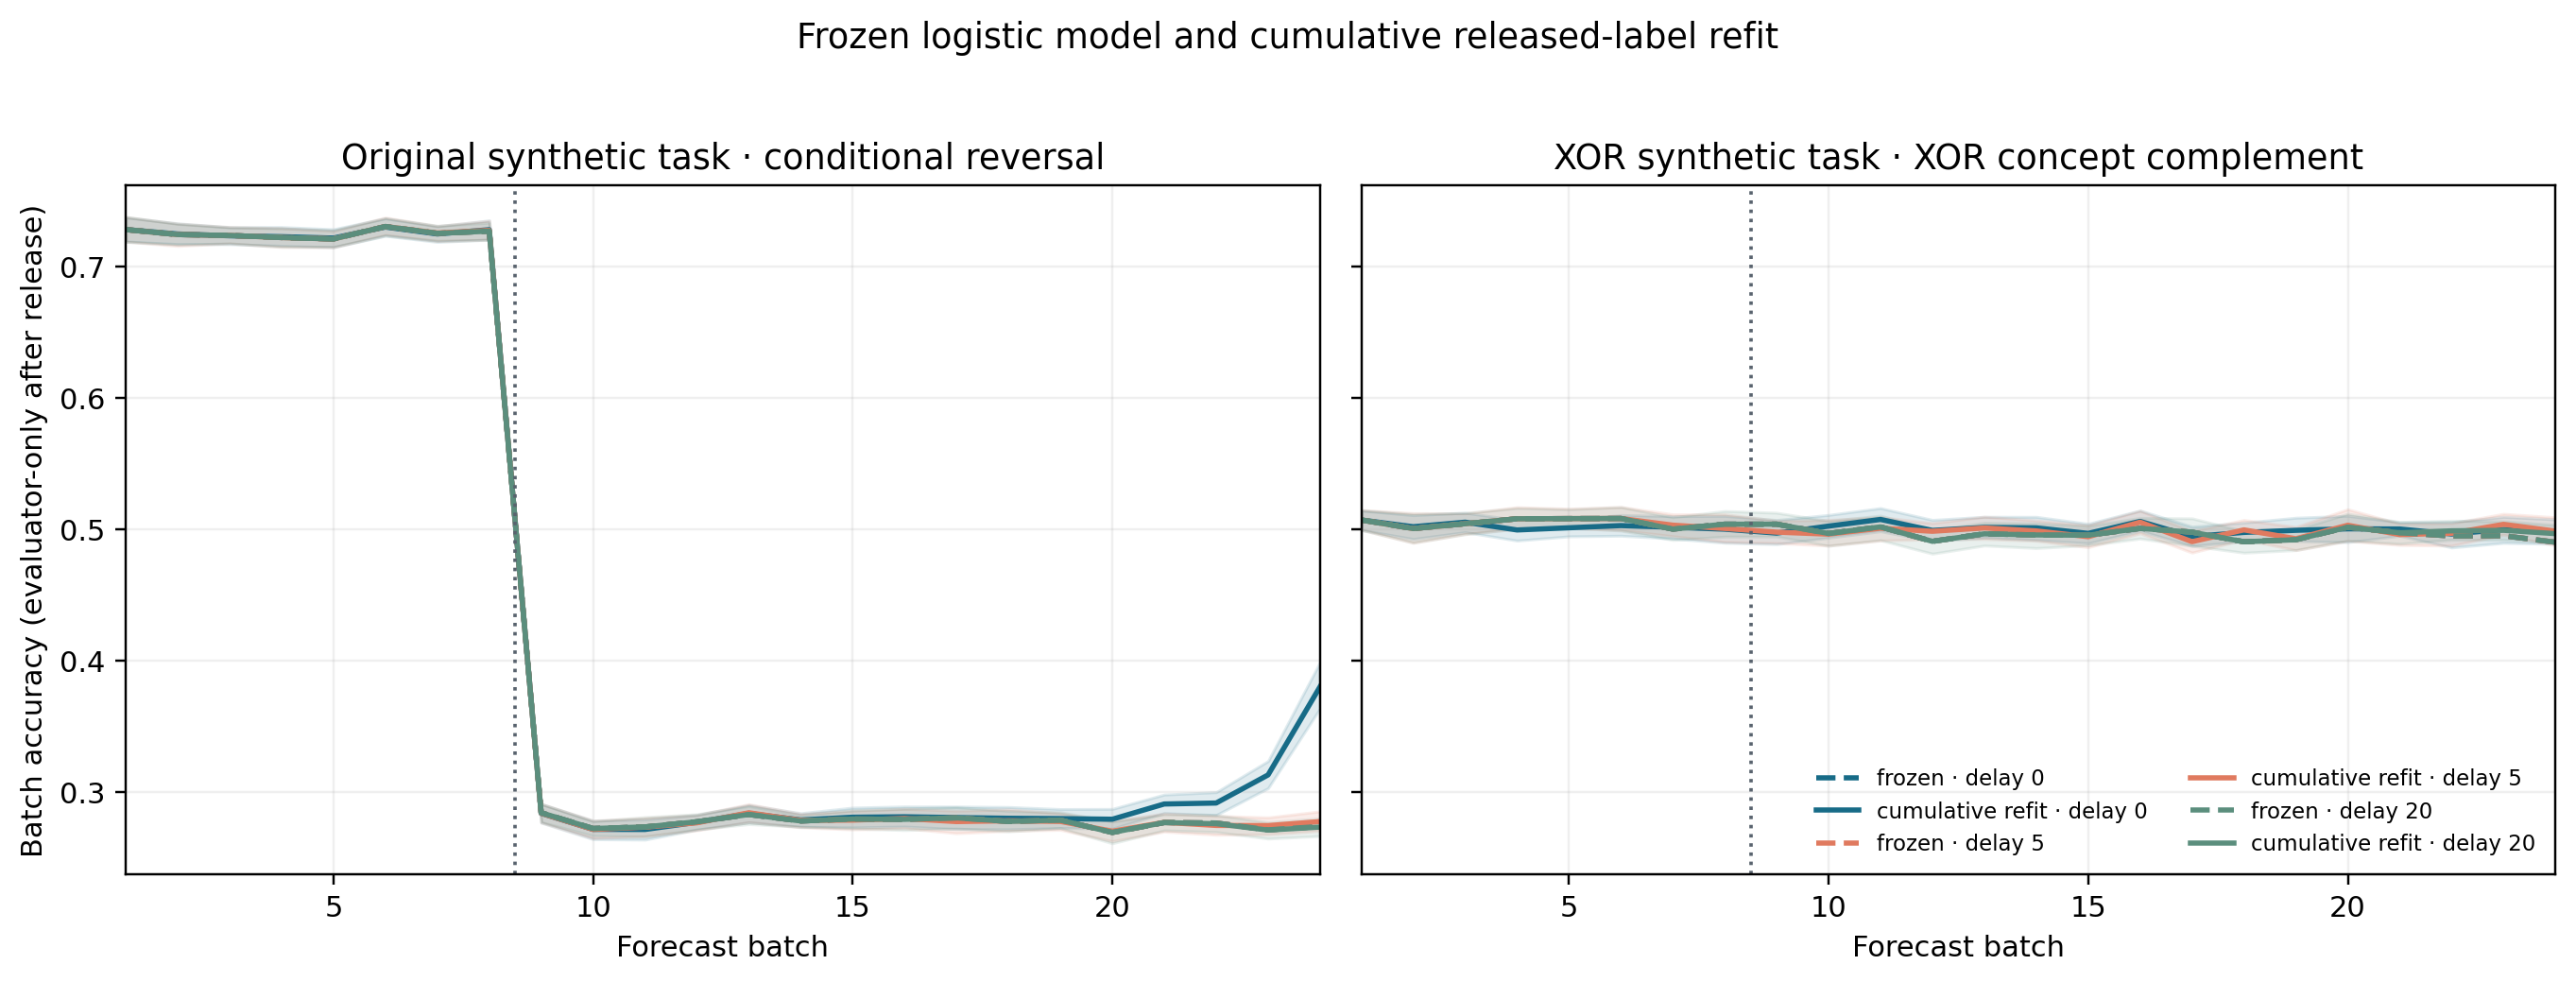
\includegraphics[width=.97\linewidth]{preserved_1_adaptation_accuracy.png}
\caption{Accuracy trajectories}
\end{figure}

\begin{figure}[htbp]\centering
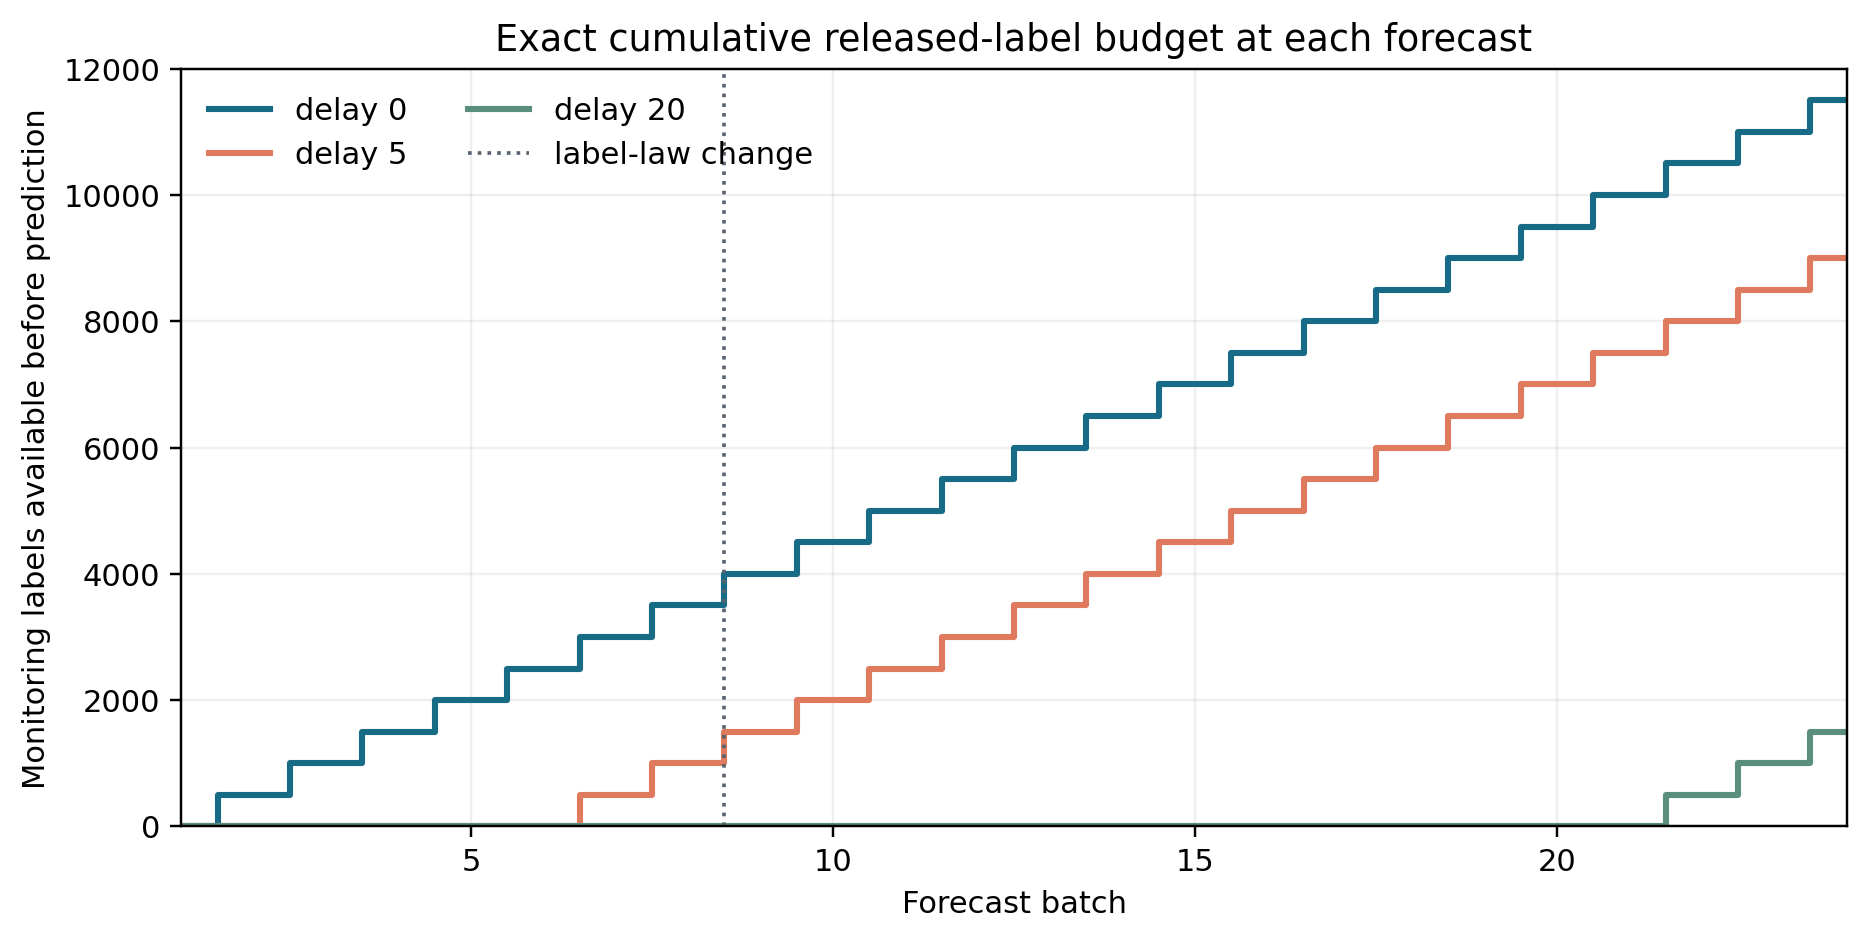
\includegraphics[width=.97\linewidth]{preserved_1_label_budgets.png}
\caption{Released-label budgets}
\end{figure}

The table reports the measured paired difference; intervals crossing zero do not establish a directional effect. C3 and X3 remain generator-specific examples. Their different results do not prove that adaptation generally repairs delayed monitoring or confidence estimation.\par

In C3 at delay 0, late post-onset accuracy rose from 0.2755 frozen to 0.2995 adapted (paired difference +0.0239); however, across all post-onset batches the paired change was only +0.0002 [-0.0007, +0.0011]. At delays 5 and 20, the late-post differences were +0.0003 and -0.0001. For X3, late-post adapted accuracy stayed near 0.50 and differences ranged from +0.0018 to +0.0034; there was no meaningful overall post-onset improvement. This is limited recovery in one condition, not a general adaptation result.\par

At the batch-24 prediction, delays 0, 5 and 20 had 11,500, 9,000 and 1,500 labels available, of which 7,500, 5,000 and 0 came from post-onset batches. Thus delay 20 had no post-onset labels available to learn from by the final input prediction. The cumulative model also retains all pre-onset training examples. A plausible explanation for the weak X3 response is that a linear logistic boundary cannot represent the XOR interaction; the experiment did not directly test alternative nonlinear update mechanisms.\par

\section{Evidence separation and validation}

An independent clean run matched 8 CSVs (17,682,084 cells) and 4,440 compressed arrays (21,840 arrays; 18,720,000 values) exactly. Timing and run-metadata fields were excluded.\par

\texttt{\seqsplit{online\_\allowbreak{}batches.csv}} and per-batch prediction archives contain no outcome fields. \texttt{\seqsplit{released\_\allowbreak{}labels.csv}} carries IDs and labels with availability clocks; \texttt{\seqsplit{evaluator\_\allowbreak{}truth/}} is retrospective. The evaluator checked exact availability budgets before each fit, that no fitting label had an availability clock at or after its forecast, same-clock persistence ordering, identical release IDs across delays, exact prediction/truth joins, and drainage without new input. All metrics are evaluator-only. This is not a security boundary or human study.\par

\section{Limitations}

This add-on studies one cumulative refit rule and one linear logistic model on two selected synthetic conditional-change cases. It does not add confidence calibration, prediction intervals, harm probabilities, or detector claims. The frozen comparison intentionally uses zero monitoring labels for fitting; only the availability schedules are shared. Cumulative retraining repeatedly reuses older released labels, so compute exposure differs from incremental training even though each adaptive run receives the same unique released IDs. No external data, natural onset labels, human participants, or analyst-benefit claims are present.\par

Reproduction: from the workspace root, run \texttt{\seqsplit{powershell -NoProfile -ExecutionPolicy Bypass -File .\textbackslash{}scripts\textbackslash{}reproduce\_\allowbreak{}phase3\_\allowbreak{}adaptation.ps1 -RunDir results/phase3/adaptation\_\allowbreak{}new\_\allowbreak{}reproduction -ReportDir reports/phase3/adaptation\_\allowbreak{}new\_\allowbreak{}reproduction}}. Use fresh, unused output directories. The wrapper evaluates the saved labels, checks exact equality with this final run, and renders the report. Exact Python package versions are in \texttt{\seqsplit{environment.json}}.\par


\section{Validation and unresolved claims}

The audit extension passed equal-quota, future-score isolation, zero-delay ordering and long-delay availability checks. Its 1,500-seed-per-task robustness replication is complete: 36,000 model streams, 864,000 online rows and 864,000 evaluator rows, with no failed seeds. A fresh five-seed sample per task reproduced 2,880 online and 2,880 evaluator rows; categorical and count fields matched exactly, and floating fields differed by at most 1.11e-16 under the recorded tight tolerance. The initial bitwise comparison failure is retained in the continuation log. This report does not claim a fresh full rerun of the earlier classifier experiments. A larger number of seeds cannot repair calibration transfer, prove future forecasting, establish causal explanations, or replace a participant study.\par

The evidence view labels unresolved estimates and current-cohort scope. Its release logic passed 75,600 boundary checks; this is not a browser usability study and does not certify current calibration. The supplementary package passed CRC and member-hash checks, five focused tests, clean-extraction reruns of the audit and horizon analyses, and exact comparisons of all ten generated result CSVs. The original Phase 2 DOCX, implementation brief and submitted archive remain preserved. New results and this manuscript are research improvements, not an uploaded replacement submission.\par


\section{Exploratory future-horizon persistence benchmark}

At input clock t, each current estimate is persisted to t+1 or t+5 without future features or labels. These are explicit forecasting baselines, not a learned future-risk model. Estimates and issue/target clocks are exported separately from truth. Methods are compared within each horizon because available cohorts differ. No future-interval guarantee is claimed. Below are C3 results; all conditions are exported.\par

\begingroup\scriptsize
\begin{longtable}{p{0.15166666666666667\linewidth}p{0.15166666666666667\linewidth}p{0.15166666666666667\linewidth}p{0.15166666666666667\linewidth}p{0.15166666666666667\linewidth}p{0.15166666666666667\linewidth}}
\toprule
condition & horizon & method & mae & bias & cohorts \\
\midrule
\endfirsthead
\toprule
condition & horizon & method & mae & bias & cohorts \\
\midrule
\endhead
C3 & 0 & ATC\_\allowbreak{}persistence & 0.304 & 0.296 & 24.000 \\
C3 & 0 & calibrated\_\allowbreak{}persistence & 0.303 & 0.297 & 24.000 \\
C3 & 0 & historical\_\allowbreak{}constant & 0.303 & 0.296 & 24.000 \\
C3 & 0 & raw\_\allowbreak{}persistence & 0.303 & 0.298 & 24.000 \\
C3 & 1 & ATC\_\allowbreak{}persistence & 0.317 & 0.309 & 23.000 \\
C3 & 1 & calibrated\_\allowbreak{}persistence & 0.315 & 0.310 & 23.000 \\
C3 & 1 & historical\_\allowbreak{}constant & 0.315 & 0.309 & 23.000 \\
C3 & 1 & raw\_\allowbreak{}persistence & 0.316 & 0.311 & 23.000 \\
C3 & 5 & ATC\_\allowbreak{}persistence & 0.379 & 0.375 & 19.000 \\
C3 & 5 & calibrated\_\allowbreak{}persistence & 0.378 & 0.375 & 19.000 \\
C3 & 5 & historical\_\allowbreak{}constant & 0.378 & 0.375 & 19.000 \\
C3 & 5 & raw\_\allowbreak{}persistence & 0.379 & 0.376 & 19.000 \\
\bottomrule
\end{longtable}
\endgroup

The external historical class-composition denominator error is corrected in separate source-versus-reference metadata, with proportions checked to sum to one within each population. Preserved original monitoring outcomes are unchanged.\par


\section{Large-seed robustness replication}

The locked robustness run completed 1,500 fresh seeds per synthetic task, covering 36,000 model streams and 864,000 online plus 864,000 evaluator batch rows. The evaluator checked separate truth, model pairing, identical input evidence, exact harm boundaries, finite values, and 2,000 seed-level bootstrap replicates; no seed failures were recorded. An independent five-seed-per-task regeneration matched 2,880 online and 2,880 evaluator rows. Discrete fields matched exactly; maximum floating-point difference was 1.11e-16 under rtol 1e-12 / atol 1e-14. This reduces seed uncertainty within the generators, not domain uncertainty.\par

\begingroup\scriptsize
\begin{longtable}{p{0.182\linewidth}p{0.182\linewidth}p{0.182\linewidth}p{0.182\linewidth}p{0.182\linewidth}}
\toprule
Task condition & Model & Accuracy [95\% seed interval] & Calibrated MAE [95\% seed interval] & Coverage [95\% seed interval] \\
\midrule
\endfirsthead
\toprule
Task condition & Model & Accuracy [95\% seed interval] & Calibrated MAE [95\% seed interval] & Coverage [95\% seed interval] \\
\midrule
\endhead
stationary original & logistic & 0.7230 [0.7228, 0.7232] & 0.0169 [0.0168, 0.0171] & 0.9270 [0.9236, 0.9302] \\
stationary original & shallow\_\allowbreak{}tree & 0.6938 [0.6934, 0.6941] & 0.0178 [0.0177, 0.0180] & 0.9251 [0.9218, 0.9284] \\
conditional-only original & logistic & 0.4257 [0.4255, 0.4259] & 0.3028 [0.3024, 0.3032] & 0.3103 [0.3086, 0.3119] \\
conditional-only original & shallow\_\allowbreak{}tree & 0.4356 [0.4354, 0.4359] & 0.2641 [0.2636, 0.2646] & 0.3085 [0.3068, 0.3102] \\
dependence original & logistic & 0.6722 [0.6720, 0.6724] & 0.0186 [0.0184, 0.0189] & 0.9164 [0.9126, 0.9203] \\
dependence original & shallow\_\allowbreak{}tree & 0.6363 [0.6360, 0.6367] & 0.0326 [0.0322, 0.0331] & 0.6789 [0.6705, 0.6877] \\
stationary XOR & logistic & 0.5004 [0.4999, 0.5009] & 0.0198 [0.0196, 0.0200] & 0.9292 [0.9259, 0.9324] \\
stationary XOR & shallow\_\allowbreak{}tree & 0.7022 [0.6936, 0.7103] & 0.0162 [0.0160, 0.0165] & 0.9279 [0.9246, 0.9311] \\
conditional-only XOR & logistic & 0.4997 [0.4994, 0.4999] & 0.0225 [0.0221, 0.0230] & 0.8880 [0.8813, 0.8941] \\
conditional-only XOR & shallow\_\allowbreak{}tree & 0.4327 [0.4299, 0.4353] & 0.2771 [0.2667, 0.2879] & 0.4567 [0.4440, 0.4692] \\
label-noise XOR & logistic & 0.5002 [0.4998, 0.5005] & 0.0202 [0.0200, 0.0204] & 0.9225 [0.9190, 0.9260] \\
label-noise XOR & shallow\_\allowbreak{}tree & 0.6181 [0.6130, 0.6231] & 0.0926 [0.0892, 0.0959] & 0.5276 [0.5133, 0.5422] \\
\bottomrule
\end{longtable}
\endgroup

The larger run retains the central failures: conditional-only changes produce no input alarms and concern flags miss harmful batches; the C6 dependence event alarms in 563/1,500 seeds; and the logistic model remains near chance on stationary XOR while the fixed tree performs better. These results sharpen the scope limits; they do not repair calibration under arbitrary change or demonstrate external validity. The supplementary robustness report contains the detailed estimation-error and interval-coverage figure.\par

\begin{figure}[htbp]\centering
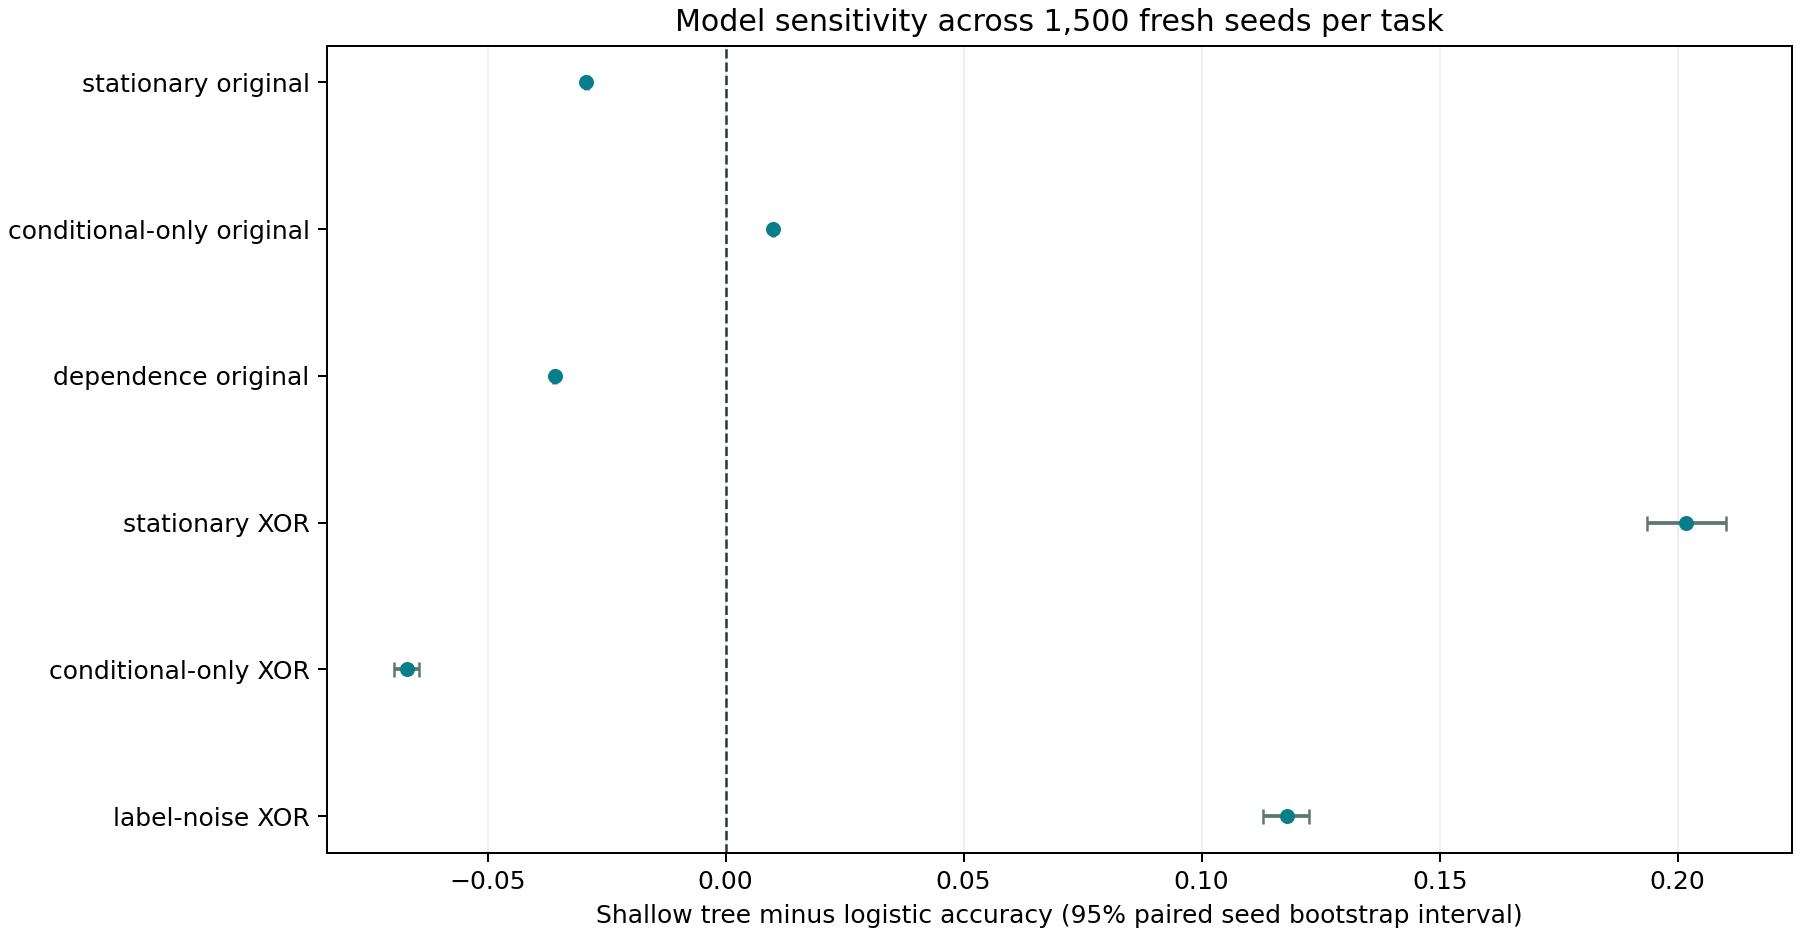
\includegraphics[width=.97\linewidth]{../large_seed_robustness_final/paired_accuracy.png}
\caption{Large-seed paired accuracy}
\end{figure}

The first independent reproduction check stopped on bitwise floating-point comparison. The comparison contract was transparently corrected: categorical and count fields remain exact, while floats use a tight tolerance. The failed first attempt is retained in the continuation logs.\par
% References and direct source links are given in Section 6.
\end{document}